\documentclass[journal]{IEEEtran}
\usepackage{amssymb}
\usepackage{amsmath}
\usepackage{graphicx}
\usepackage{textcomp}
\usepackage{xcolor}
\usepackage{tabularx}
\usepackage{braket}
\usepackage{booktabs}
\usepackage{tikz}
\usepackage{bm}
\usepackage{caption}
\usepackage{subcaption}
\usepackage{pifont,array} %For ding
\usepackage{multicol}
\usepackage{multirow}
\usepackage{nccmath}
\usepackage{xurl}
\usepackage{xspace}
\usepackage{comment}
\usepackage{makecell, kotex}
\usepackage{hyperref}
\usepackage{colortbl}
\usepackage[most]{tcolorbox} 
\usepackage{algorithm}
\usepackage[noend]{algpseudocode}  % noend 옵션 추가

\usepackage{titlesec}
\titlespacing{\subsection}{0pt}{1pt}{0pt}
\titlespacing{\section}{0pt}{2pt}{1pt}
\setlength{\baselineskip}{8pt}
\captionsetup{font=small}
\setlength{\textfloatsep}{1pt plus 1.0pt minus 1.0pt}
\setlength{\floatsep}{1pt plus 1pt minus 1pt}
\setlength{\intextsep}{1pt plus 1pt minus 1pt}
\DeclareUnicodeCharacter{2713}{\checkmark}


\definecolor{pred}{rgb}{0.7843, 0.0039, 0.3137}
\definecolor{dblue}{rgb}{0.0, 0.0, 1.0}
\definecolor{sorange}{rgb}{0.91, 0.45, 0.32}
\newcommand{\skim}[1]{{\color{sorange}{#1}}} %
\newcommand{\changjong}[1]{{\color{pred}{#1}}}
    

\usetikzlibrary{fit,shapes,arrows,positioning}

%% Commands
\newcommand{\edgeQsim}{\texttt{EdgeQuantum}\xspace}
\newcommand{\EdgeQuantum}{\texttt{EdgeQuantum}\xspace}



\newcommand{\cmark}{{\color{green!70!black}\ding{51}}}
\newcommand{\xmark}{{\color{red!80!black}\ding{55}}}
\newcommand{\pmark}{{\color{orange!80!black}$\triangle$}}

\begin{document}

\title{\edgeQsim: Quantum Circuit Simulation Framework for Resource-Constrained Edge Devices}

\author{Changjong Kim, Ehan Sohn and Sunggon Kim
\thanks{Changjong Kim, Ehan Sohn, and Sunggon Kim are with the Department of Computer Science and Engineering, Seoul National University of Science and Technology, 232, Gongneung-ro, Nowon-gu, Seoul, Republic of Korea (e-mail: changjong5238@seoultech.ac.kr; ehanjsohn@seoultech.ac.kr; sunggonkim@seoultech.ac.kr).}
}

\maketitle
\begin{abstract}
This paper presents \EdgeQuantum, a tiered-memory quantum circuit simulator designed to overcome the memory wall of resource-constrained edge devices. As quantum algorithms scale toward dozens of qubits for on-device verification of NISQ workloads, simulating their state vectors on edge devices demands coordinated multi-tier memory management beyond the device's physical DRAM capacity. \EdgeQuantum introduces a unified storage hierarchy that integrates GPU VRAM, unified DRAM, and external NVMe storage. With this design, \EdgeQuantum achieves zero-copy data movement across tiers through UVM-based attach toggling, hides write latency through a 4-buffer asynchronous pipeline with serialized NVMe access, and expands effective storage capacity through ping-pong LZ4 compression. Our evaluation across six quantum circuits on an 8\,GB NVIDIA Jetson Orin Nano shows that \EdgeQuantum enables 39-qubit (4\,TB) state-vector simulation, outperforming blocking I/O baselines by up to 1.48$\times$ while expanding effective memory capacity by 512$\times$.
\end{abstract}

\begin{IEEEkeywords}
Quantum Computing, Quantum Circuit Simulation, Edge Computing, GPU Acceleration, cuQuantum, Tiered Memory
\end{IEEEkeywords}

\section{Introduction}
\label{sec:intro}


Quantum computing offers a computational model distinct from classical computing by operating on qubits rather than binary bits. Each qubit is represented as a quantum state with probability amplitudes (e.g., $|\psi\rangle = \alpha|0\rangle + \beta|1\rangle$), where superposition enables multiple states, and entanglement creates correlations between qubits. These properties enable parallelism beyond classical computation~\cite{renner2022computational, miguel2023enhancing}. Despite these advantages, current quantum computers remain limited to Noisy Intermediate-Scale Quantum (NISQ) devices with high error rates and short coherence times~\cite{lau2022nisq, saki2019study, preskill2018quantum}. To validate algorithms without hardware-induced errors, classical computers are used for quantum circuit simulation. Specifically, full state vector simulation evaluates all probability amplitudes to provide the exact state distributions and precise gradients essential for training quantum machine learning models~\cite{miller2025phase2, kim2023evidence, xu2025herculean}. 

While full state vector simulation guarantees exact results, its exponential memory footprint forces existing frameworks to rely on state-of-the-art infrastructures, including HPC and cloud systems equipped with terabytes of memory and high-performance GPU clusters~\cite{xu2024atlas, 10.1145/3771577, zhang2021hyquas}. However, as quantum applications transition to real-world deployments (e.g., decentralized quantum sensor networks~\cite{guo2020distributed}, privacy-sensitive medical IoT~\cite{barua2024data}, and autonomous robotics~\cite{skolik2022quantum}), relying on such centralized infrastructures becomes impractical for data-intensive edge workloads~\cite{fernandez2019pre, caro2022generalization}. First, regulated data (e.g., HIPAA-protected medical telemetry, GDPR-protected biometrics) is legally restricted from leaving the device~\cite{theodos2020health, khan2021federated}. Second, field-deployed nodes operate beyond reliable network coverage~\cite{wang2020convergence, lim2020federated}. Third, relying on centralized high-end computing resources incurs prohibitive infrastructure costs across thousands of IoT devices~\cite{xu2024iot, gill2019transformative}. Finally, emerging applications such as hybrid quantum-classical machine learning and Variational Quantum Algorithms (VQAs) over IoT sensor streams require thousands of iterative circuit executions~\cite{verma2025quantum, cerezo2021variational, mastroianni2024variational}. Offloading this optimization process to the cloud incurs network round-trips on every iteration, where communication latencies quickly accumulate into hours of idle blocking time. Therefore, quantum parameters must be optimized on the device that generates the data~\cite{zhang2025breaking, li2025infscaler}.


However, edge-native quantum simulation is fundamentally constrained by an exponential memory wall. The footprint of a quantum state vector grows exponentially, rapidly exceeding the strict physical memory limits of edge SoCs (e.g., 8 GB on an NVIDIA Jetson Orin Nano~\cite{jetson_orin_nano}). Furthermore, unlike servers equipped with discrete GPUs, edge devices employ a Unified Memory Architecture (UMA) where the CPU, GPU, and operating system share a single DRAM pool. When a massive state vector exhausts the shared environment, it starves essential system workspaces, leading to execution bottlenecks and out-of-memory (OOM) failures.


%To overcome this memory barrier, existing approaches attempt to deploy high-performance frameworks (e.g., cuQuantum) using out-of-core memory management. However, applying these frameworks to edge environments exposes an architecture mismatch. In contrast to discrete GPUs, edge devices employ a Unified Memory Architecture (UMA) where the CPU and GPU share a constrained physical memory pool. When standard frameworks attempt to allocate large state vectors within this shared pool, they exhaust the available DRAM. Lacking edge-aware memory management, they fall back on operating system virtual memory (OS-native swapping) to spill data to external NVMe storage, which triggers I/O thrashing. Figure~\ref{intro_motivation_b} shows the impact of this mismatch on a Variational Quantum Eigensolver (VQE) workload. CPU-only execution (Cirq) avoids GPU memory exhaustion but is computationally expensive, requiring over 100 seconds (109,168ms) for a single 29-qubit iteration. Conversely, GPU-accelerated execution (cuQuantum) degrades as it triggers OS swapping near physical memory limits (96.6ms at 29 qubits), before crashing with an Out-of-Memory (OOM) error at 30 qubits due to GPU workspace overheads and CUDA allocator constraints. In contrast, \EdgeQuantum leverages a UMA-optimized architecture to bypass OS bottlenecks, maintaining millisecond-level latency (2.0~ms) at 29 qubits and completing the 30-qubit out-of-core simulation in 10.3 seconds.

\begin{table}[t]
\caption{Comparison with prior work across key capabilities (TA: Tiered Architecture, CS: Compression Support, MN: Multinode Support, UO: UMA Optimization, RS: Reported Scale).}
\vspace{-.2cm}

\centering
\scriptsize
\begin{tabularx}{\columnwidth}{p{1.8cm}|c|c|c|c|c|c|c}
\toprule
\textbf{Framework} & \textbf{Target} & \textbf{GPU} & \textbf{TA} & \textbf{CS} & \textbf{MN} & \textbf{UO} & \textbf{RS} \\
\midrule
Google Cirq~\cite{cirq} & General &  &  &  & \checkmark &  & 32 \\
Qiskit Aer~\cite{qiskit_aer} & General & \checkmark &  &  &  &  & 32+ \\
Google Qsim~\cite{qsim} & General & \checkmark &  &  & \checkmark &  & 32+ \\
cuQuantum~\cite{bayraktar2023cuquantum} & General & \checkmark &  &  & \checkmark &  & 32+ \\
PennyLane~\cite{pennylane} & General & \checkmark &  &  & \checkmark &  & 32+ \\
HyQuas~\cite{zhang2021hyquas} & HPC system & \checkmark &  &  &  &  & 36 \\
Atlas~\cite{xu2024atlas} & HPC system & \checkmark & &  & \checkmark &  & 36 \\
ScaleQsim~\cite{10.1145/3771577} & HPC system & \checkmark &  &  & \checkmark &  & 42 \\
SnuQS~\cite{park2022snuqs} & Datacenter & \checkmark & \checkmark &  &  &  & 42 \\
BMQSim~\cite{zhang2025bmqsim} & Datacenter & \checkmark & \checkmark & \checkmark & \checkmark &  & 36 \\
\textbf{EdgeQuantum} & \textbf{Edge/IoT} & \checkmark & \checkmark & \checkmark &  & \checkmark & \textbf{39} \\
\bottomrule
\end{tabularx}
\label{intro_table}
\end{table}

Many previous studies, as summarized in Table~\ref{intro_table}, optimize quantum circuit simulation for different computing infrastructures, ranging from general-purpose workstations to HPC systems. Standard frameworks target general computing environments. While some of these frameworks support multi-node scaling through external integration, they typically assume that the state vector fits entirely within physical GPU VRAM or host DRAM~\cite{cirq, qiskit_aer, qsim, bayraktar2023cuquantum, pennylane}. Several works target HPC systems and use multi-node execution to scale memory capacity, but they rely heavily on high-bandwidth interconnects such as NVLink and InfiniBand~\cite{xu2024atlas, 10.1145/3771577, zhang2021hyquas}. Other works leverage tiered memory and out-of-core data compression for datacenter environments, but target server-grade GPUs~\cite{park2022snuqs, zhang2025bmqsim}. Specifically, while \textit{BMQSim}~\cite{zhang2025bmqsim} scales capacity through tiered memory pipelines, it does not provide the UMA-aware optimizations required to eliminate redundant memory copies on shared-memory edge SoCs. Thus, these existing approaches do not consider the hardware characteristics of edge systems, including restricted NVMe bandwidth and the physical constraints of Unified Memory Architecture (UMA), where traditional host-driven I/O pipelines saturate the memory controller.


In this paper, we present \EdgeQuantum, a scalable full state-vector simulation framework for resource-constrained edge devices. While existing out-of-core simulators address memory limitations through OS-native swapping or server-grade abstractions, they do not coordinate the end-to-end I/O path for UMA environments. \EdgeQuantum integrates unified DRAM and commodity NVMe storage into a 2-tier memory architecture that decouples logical state-vector management from physical residency. Specifically, \EdgeQuantum introduces 1) an out-of-core state vector chunking mechanism that extends logical capacity to NVMe storage beyond hardware limits, 2) an edge-aware asynchronous Unified Virtual Memory (UVM) pipeline that serializes storage access and overlaps flash operations with GPU computation, and 3) an on-the-fly mantissa-truncated LZ4 ping-pong compression strategy that circumvents in-place update limitations through dual-file alternation, achieving up to 255$\times$ per-file compression. Our evaluation on an 8GB Jetson Orin Nano demonstrates that \EdgeQuantum supports up to a 39-qubit simulation (4TB footprint) and achieves a 512$\times$ logical capacity expansion beyond physical DRAM. We open-source \EdgeQuantum at \url{https://github.com/sunggonkim/IoTJ-EdgeQuantum}





%Specifically, \EdgeQuantum introduces 1) state vector partitioning across shared DRAM and NVMe to enable large-scale simulations beyond hardware limits, 2) an edge-aware asynchronous Unified Virtual Memory (UVM) pipeline that serializes storage access to avoid I/O contention and overlaps flash operations with GPU computation, and 3) an on-the-fly LZ4 ping-pong compression strategy that bypasses the impossibility of in-place updates for variable-sized data by alternating backing files, thereby expanding effective storage capacity by $242.7\times$ while masking NVMe latency.
\section{Background}

\begin{figure}[t]
    \centering
    \begin{subfigure}[b]{0.46\columnwidth}
        \centering
        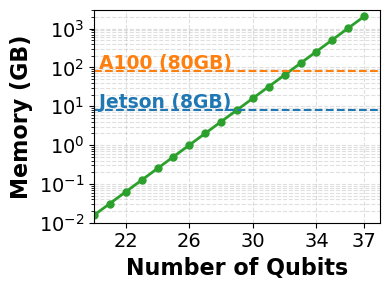
\includegraphics[width=\linewidth]{Figures/fig_motivation_a.png}
        \caption{Memory growth.}
        \label{intro_motivation_a}
    \end{subfigure}\hfill
    \begin{subfigure}[b]{0.50\columnwidth}
        \centering
        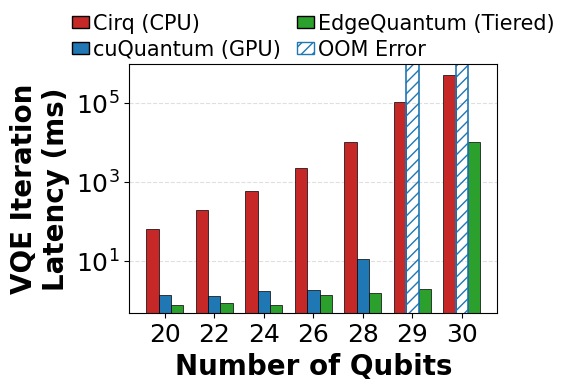
\includegraphics[width=\linewidth]{Figures/fig_motivation_b.png}
        \caption{VQE latency.}
        \label{intro_motivation_b}
    \end{subfigure}
    \caption{Memory wall and per-iteration VQE latency on resource-constrained edge devices.}
    \label{intro_motivation}
\end{figure}

\subsection{GPU-Accelerated Quantum Circuit Simulation}\label{back1}
Quantum circuit simulation involves trade-offs between scalability and computational complexity~\cite{qsim, svsim, suzuki2021qulacs, villalonga2019flexible}. Tensor network contraction reduces memory usage, but its computational cost grows exponentially for highly entangled circuits~\cite{gray2018quimb, lykov2022tensor, pan2022simulation}. In contrast, full state vector simulation explicitly maintains every probability amplitude, providing exact results regardless of circuit depth or entanglement structure~\cite{guerreschi2020intel, de2007massively, qsim, suzuki2021qulacs}. To process these vectors, simulators like \textit{cuStateVec}~\cite{bayraktar2023cuquantum} and \textit{Qiskit Aer}~\cite{qiskit} rely on GPU acceleration. They allocate the state vector in VRAM and process the circuit layer by layer, where CUDA kernels apply quantum gates in parallel, and data remains on-device, avoiding intermediate transfers.

\noindent\textbf{Memory Wall. }GPU-accelerated full state vector simulation is fundamentally limited by memory capacity. Memory footprint grows exponentially with the number of qubits at a complexity of $\mathcal{O}(2^n)$. Since each complex amplitude requires 8 bytes in single precision, a 30-qubit circuit demands 8GB, exhausting the 8GB limit of edge devices such as the NVIDIA Jetson Orin Nano. Scaling further, a 34-qubit circuit requires 128GB, and a 39-qubit circuit demands 4TB, far exceeding edge memory capacities. As shown in Figure~\ref{intro_motivation_a}, this exponential growth defines the memory wall on edge devices, while server-grade discrete GPUs such as the NVIDIA A100 sustain in-memory execution up to 80GB of dedicated VRAM. The wall is further amplified by the unified memory architecture: the 8GB physical DRAM is shared by the OS, CPU, and GPU, leaving insufficient headroom for kernel workspaces and runtime allocations once the state vector approaches the limit. 

\noindent\textbf{Per-iteration VQE Latency. }As shown in Figure~\ref{intro_motivation_b}, this memory wall manifests as the qubit count grows on edge devices. CPU-only execution (\textit{Cirq}) avoids GPU workspace overhead but pays orders-of-magnitude compute cost, requiring over 100 seconds (109,168ms) for a single 29-qubit VQE iteration. GPU-accelerated execution (\textit{cuQuantum}) fails to simulate 29 qubits, immediately crashing with an Out-of-Memory (OOM) error due to physical memory capacity constraints. To address this, out-of-core memory management is required. Existing frameworks~\cite{zhang2025bmqsim, wu2019full, li2021sv, park2022snuqs} employ data compression and tiered memory pipelines to mitigate memory limits. However, these approaches are optimized for server-grade GPUs with discrete PCIe topologies and abundant host resources. Adapting them to edge environments requires falling back to blocking I/O on external NVMe storage. Their pipelines assume host-driven DMA paths that are absent on UMA SoCs, stalling GPU computation and incurring severe I/O latency. In contrast, \EdgeQuantum resolves these bottlenecks through a UMA-aware asynchronous pipeline that prevents OOM failures and effectively masks I/O latency through pipeline overlap and on-the-fly compression, demonstrating stable and high-performance execution across the memory wall.





\subsection{Memory Architecture in Edge Computing}\label{back2}

\begin{figure}[t]
    \centering
    \begin{subfigure}[b]{\columnwidth}
        \centering
        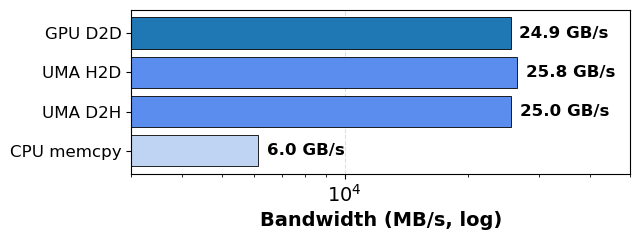
\includegraphics[width=\linewidth]{Figures/edge_back2.png}
        \caption{Unified DRAM (LPDDR5).}
        \label{fig:bg_bw_dram}
    \end{subfigure}

    \vspace{0.5em}

    \begin{subfigure}[b]{\columnwidth}
        \centering
        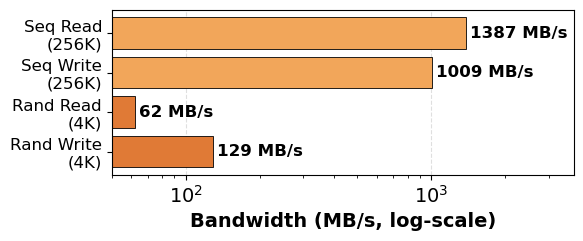
\includegraphics[width=\linewidth]{Figures/edge_back3.png}
        \caption{External NVMe SSD.}
        \label{fig:bg_bw_nvme}
    \end{subfigure}
    \vspace{-.2cm}

    \caption{Bandwidth across the edge memory hierarchy on the Jetson Orin Nano. Unified DRAM bandwidth is measured via CUDA memory copy operations. External NVMe SSD bandwidth is evaluated using FIO~\cite{} with \texttt{O\_DIRECT} (256~KB blocks for sequential and 4~KB blocks for random accesses).}
    \label{fig:bg_bandwidth}
    \vspace{-.2cm}
\end{figure}

To handle data-intensive applications such as quantum simulation on edge devices, it is necessary to understand the underlying memory architecture. Unlike HPC clusters that use discrete CPUs and GPUs connected via PCIe, edge devices such as the NVIDIA Jetson Orin Nano use a System-on-Chip (SoC) design with a Unified Memory Architecture (UMA)~\cite{nvidia2022jetson}. In this architecture, the CPU and GPU share a single physical DRAM pool, eliminating PCIe data transfers. However, this integrated design introduces bandwidth asymmetry depending on the access path and storage tier.

\noindent\textbf{Unified Memory Architecture. }
As shown in Figure~\ref{fig:bg_bw_dram}, within LPDDR5 DRAM, GPU-driven and UMA transfers (e.g., GPU D2D, UMA H2D/D2H) deliver about 25~GB/s, whereas host-driven CPU memory copies achieve only 6.0~GB/s. This is a 4$\times$ difference within the same physical memory. Recent studies in large-scale data processing propose out-of-core mechanisms~\cite{lin2022hm, hwang2020centaur} that use a user-space buffer manager to prefetch data and overlap I/O with computation. However, applying these techniques to quantum simulation on unified memory architectures presents challenges. Existing frameworks assume separate memory spaces and rely on host-driven staging. This causes their data movement to be limited by the 6.0~GB/s CPU memcpy rate, failing to exploit the higher UMA bandwidth.

\noindent\textbf{External Storage Device. }
As shown in Figure~\ref{fig:bg_bw_nvme}, when data moves to the external NVMe SSD, bandwidth decreases significantly. Sequential reads and writes provide about 1.38~GB/s and 1.0~GB/s. This is an 18$\times$ reduction compared to UMA transfers. Small-block random accesses reduce bandwidth further to 62~MB/s, which is a 400$\times$ reduction. Existing out-of-core approaches rely on operating system virtual memory management (OS-native swapping) to handle data larger than physical memory. However, the OS memory manager does not consider quantum gate access patterns, where memory stride increases exponentially with the target qubit index. Because this strided access pattern defeats standard OS readahead heuristics, page faults generate small-block storage accesses. This forces the NVMe drive into the random read state, reducing bandwidth to 62~MB/s. Consequently, this gap between the GPU kernel and OS file system leads to I/O thrashing and low GPU utilization. Furthermore, the physical storage capacity is limited to approximately 256~GB, which is insufficient to store raw state vectors of 35 qubits or more ($\geq256$~GB).

Optimizing quantum simulation on edge devices requires a specialized memory management strategy. The design must use zero-copy capabilities of UMA to sustain 25~GB/s bandwidth. It must enforce large sequential NVMe accesses (1.38~GB/s) to avoid the 62~MB/s random I/O penalty. \EdgeQuantum implements a UVM-aware asynchronous pipeline. It combines sequential I/O scheduling with zero-copy computation and maintains performance when the state vector exceeds physical memory capacity.
\section{\EdgeQuantum Design}
\label{sec:design}

%In this section, we present the design of \EdgeQuantum, a tiered-memory quantum circuit simulator specifically optimized for resource-constrained edge devices. 
%\EdgeQuantum overcomes the physical memory limitations of edge hardware not by simplifying the quantum circuit, but by implementing a hierarchical memory management system that treats NVMe SSD as a direct extension of the GPU memory.
%By utilizing Unified Virtual Memory (UVM) as a zero-copy staging buffer and implementing a 4-buffer asynchronous pipeline, \EdgeQuantum enables the simulation of state vectors up to 4\,TB (39 qubits) on devices with only 8\,GB of RAM.


\begin{figure}[t]
    \centering
    % Ensure you have this file or use a placeholder
    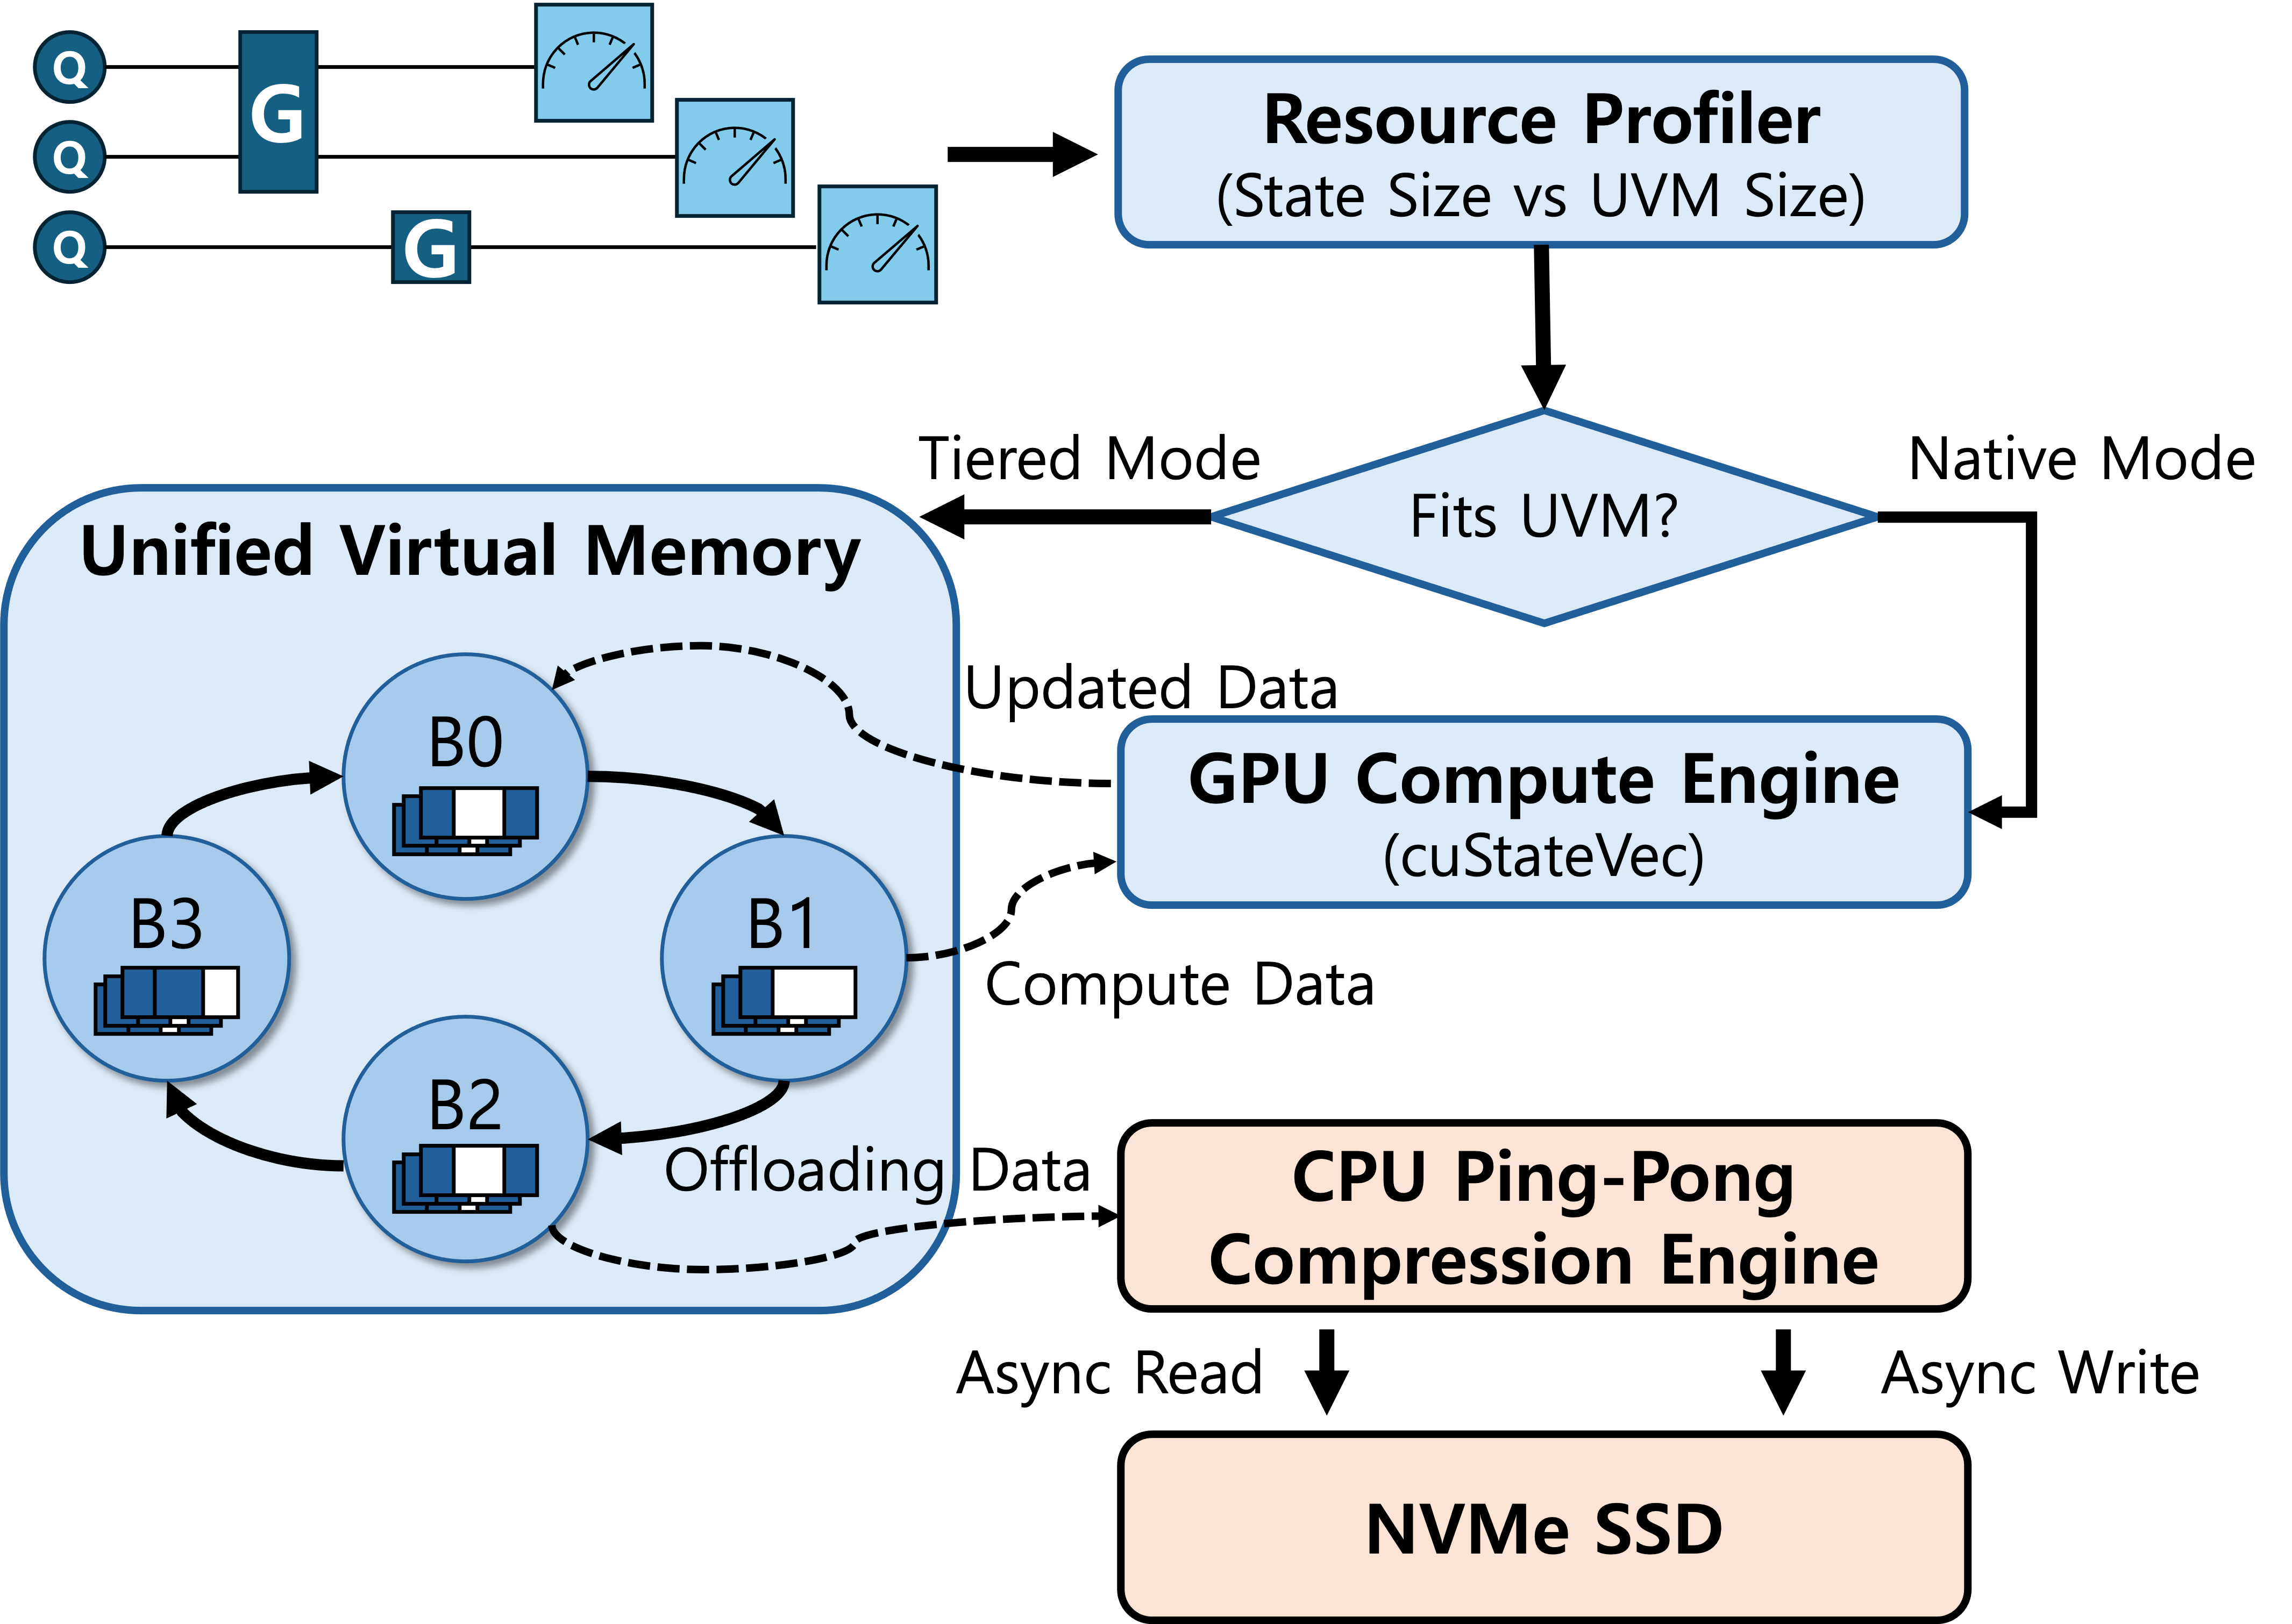
\includegraphics[width=0.85\columnwidth]{Figures/architecture_edge.png}
    \caption{Overall architecture of \EdgeQuantum.}
        \vspace{-.2cm}
    \label{overall_architecture}
\end{figure}



\subsection{Overall Procedure}
\label{design_overall}

Figure~\ref{overall_architecture} shows the overall procedure of \EdgeQuantum.
\EdgeQuantum processes a quantum circuit simulation through dynamic resource profiling and a Unified Virtual Memory (UVM)-based storage pipeline.

\noindent\textbf{Resource Profiling and Mode Selection.}
When a quantum circuit simulation starts, \textit{Resource Profiler} computes the state vector size and compares it with available memory. To prevent mid-execution out-of-memory (OOM) crashes, this comparison uses 80\% of available GPU memory as a threshold, reserving headroom for kernel workspaces and runtime allocations. Based on this comparison, \EdgeQuantum determines whether the state vector fits within available memory. If the state vector fits within available memory, \EdgeQuantum operates in \textit{Native Mode}. In this mode, \textit{GPU Compute Engine} allocates the state in memory and executes the simulation using \textit{cuStateVec}. If the state vector exceeds available memory, \EdgeQuantum activates \textit{Tiered Mode}, which uses NVMe SSD as a memory hierarchy extension. By selecting the execution path based on capacity, \EdgeQuantum utilizes available hardware and prevents OOM failures.

\noindent\textbf{Tiered Mode Execution.}
In \textit{Tiered Mode}, \EdgeQuantum employs a 4-buffer UVM pipeline that establishes a zero-copy data path through the Unified Memory Architecture (UMA), avoiding host-to-device overheads of existing simulators. The state vector is partitioned into fixed-size chunks staged through four UVM ring buffers (B0-B3). During execution, \textit{GPU Compute Engine} applies gates on UVM ring buffers, while \textit{CPU Ping-Pong Compression Engine} performs async I/O between NVMe SSD and buffers. The 4-buffer depth absorbs NVMe's asymmetric read/write latency by overlapping GPU compute on one buffer with CPU I/O on others, preventing pipeline stalls. The compression engine engages dual-file ping-pong compression when the state vector exceeds SSD capacity ($\geq$36 qubits), enabling \EdgeQuantum to simulate quantum systems (e.g., 39 qubits) that exceed physical storage capacity.



\subsection{Tiered Memory Architecture with UVM}
\label{design_memory}



A fundamental challenge in edge out-of-core simulation is the redundant host-to-device copies imposed by standard CUDA frameworks. On NVIDIA Jetson platforms, the CPU and GPU share a DRAM pool under UMA, enabling zero-copy data paths. Figure~\ref{uvm_diff} shows how \EdgeQuantum leverages UMA via UVM visibility control to establish an efficient data path.

\noindent\textbf{Existing Storage-backed Execution. }Despite the shared DRAM on UMA platforms, existing quantum simulation frameworks rely on standard device memory allocation models. As shown at the top of Figure~\ref{uvm_diff}, using standard device memory allocation (e.g., \texttt{cudaMalloc}) enforces a logical separation between host and device memory spaces. When retrieving state vector chunks from storage, POSIX I/O system calls (e.g., \texttt{pread}) cannot perform Direct Memory Access (DMA) into device memory. The system stages the data in an intermediate host-side buffer, followed by an explicit \texttt{cudaMemcpy} (H2D). This data path has two limitations for resource-constrained edge devices. First, it doubles the physical memory footprint (2$\times$ Memory constraint). Second, the additional memory copy operation saturates memory bandwidth and reduces simulation throughput.


\begin{figure}[t]
    \centering
    % Ensure you have this file or use a placeholder
    \includegraphics[width=0.85\columnwidth]{Figures/test_uvm.png}
    \caption{Data path comparison. (Top) Existing execution. (Bottom) \EdgeQuantum's zero-copy execution on UMA.}
    \vspace{-.2cm}
    \label{uvm_diff}
\end{figure}

\noindent\textbf{Zero-copy Execution for UMA. }To remove this bottleneck, \EdgeQuantum designs a zero-copy data path by controlling the visibility of UVM at the OS and driver level. As shown at the bottom of Figure~\ref{uvm_diff}, \EdgeQuantum allocates simulation buffers using \texttt{cudaMallocManaged} with the \texttt{cudaMemAttachHost} flag. This flag maps physical pages into the CPU page tables. With CPU-side visibility, \EdgeQuantum performs \texttt{O\_DIRECT} file operations, streaming state vector chunks directly into the UVM ring buffer while bypassing the Linux page cache and avoiding memory pollution. Before quantum gate execution, \EdgeQuantum issues a \texttt{cudaStreamAttachMemAsync} with \texttt{cudaMemAttachGlobal} flag. This asynchronous operation updates the GPU Memory Management Unit (MMU) page tables without data migration and transfers ownership of the physical DRAM pages to \textit{GPU Compute Engine}. By managing these UVM visibility transitions within a ring-buffer structure, \EdgeQuantum ensures that active data residency remains within physical DRAM limits, thereby preventing OS-level thrashing and removing explicit memory copies.



\subsection{4-Buffer Asynchronous Pipeline}
\label{design_pipeline}



%The primary performance bottleneck in out-of-core quantum simulation on edge devices is the asymmetric I/O latency of commodity NVMe SSDs. While sequential reads sustain 1.38~GB/s, writes are limited to 1.0~GB/s (Section~\ref{back2}). Traditional out-of-core simulators issue concurrent asynchronous reads and writes without considering this asymmetry. This bidirectional I/O causes NVMe controller contention and degrades throughput. To mitigate this hardware limitation, \EdgeQuantum implements an asynchronous pipeline governed by an \textit{I/O Serialization Policy}. 

The primary bottleneck in out-of-core quantum simulation on edge devices is the asymmetric I/O latency of NVMe SSDs (Section~\ref{back2}). Existing simulators issue concurrent reads and writes, ignoring this asymmetry. This bidirectional I/O causes controller contention and degrades throughput. To mitigate this, \EdgeQuantum implements an asynchronous pipeline with an \textit{I/O Serialization Policy}. 

\noindent\textbf{Pipeline Architecture.} Figure~\ref{design_3.3} shows the execution timeline of the asynchronous pipeline. The core design principle is to isolate I/O directions to preserve NVMe bandwidth while overlapping them with independent GPU computation. This isolation is enforced by an I/O serialization barrier, ensuring a new read is blocked until the preceding write completes. This 4-buffer configuration is selected based on the latency relationship between NVMe writes ($T_{write} \approx 256$ms for a 256 MB chunk at the measured 1.0 GB/s) and the combined read-compute window ($T_{read} + T_{compute}$). We adopt a 4-buffer depth to provide headroom against write-latency variability, ensuring a free UVM ring buffer is available for the next $T_{read}$ phase. Driven by this policy, \EdgeQuantum processes state vector chunk $k$ through the following sequence:

\begin{figure}[t]
    \centering
    % Ensure you have this file or use a placeholder
    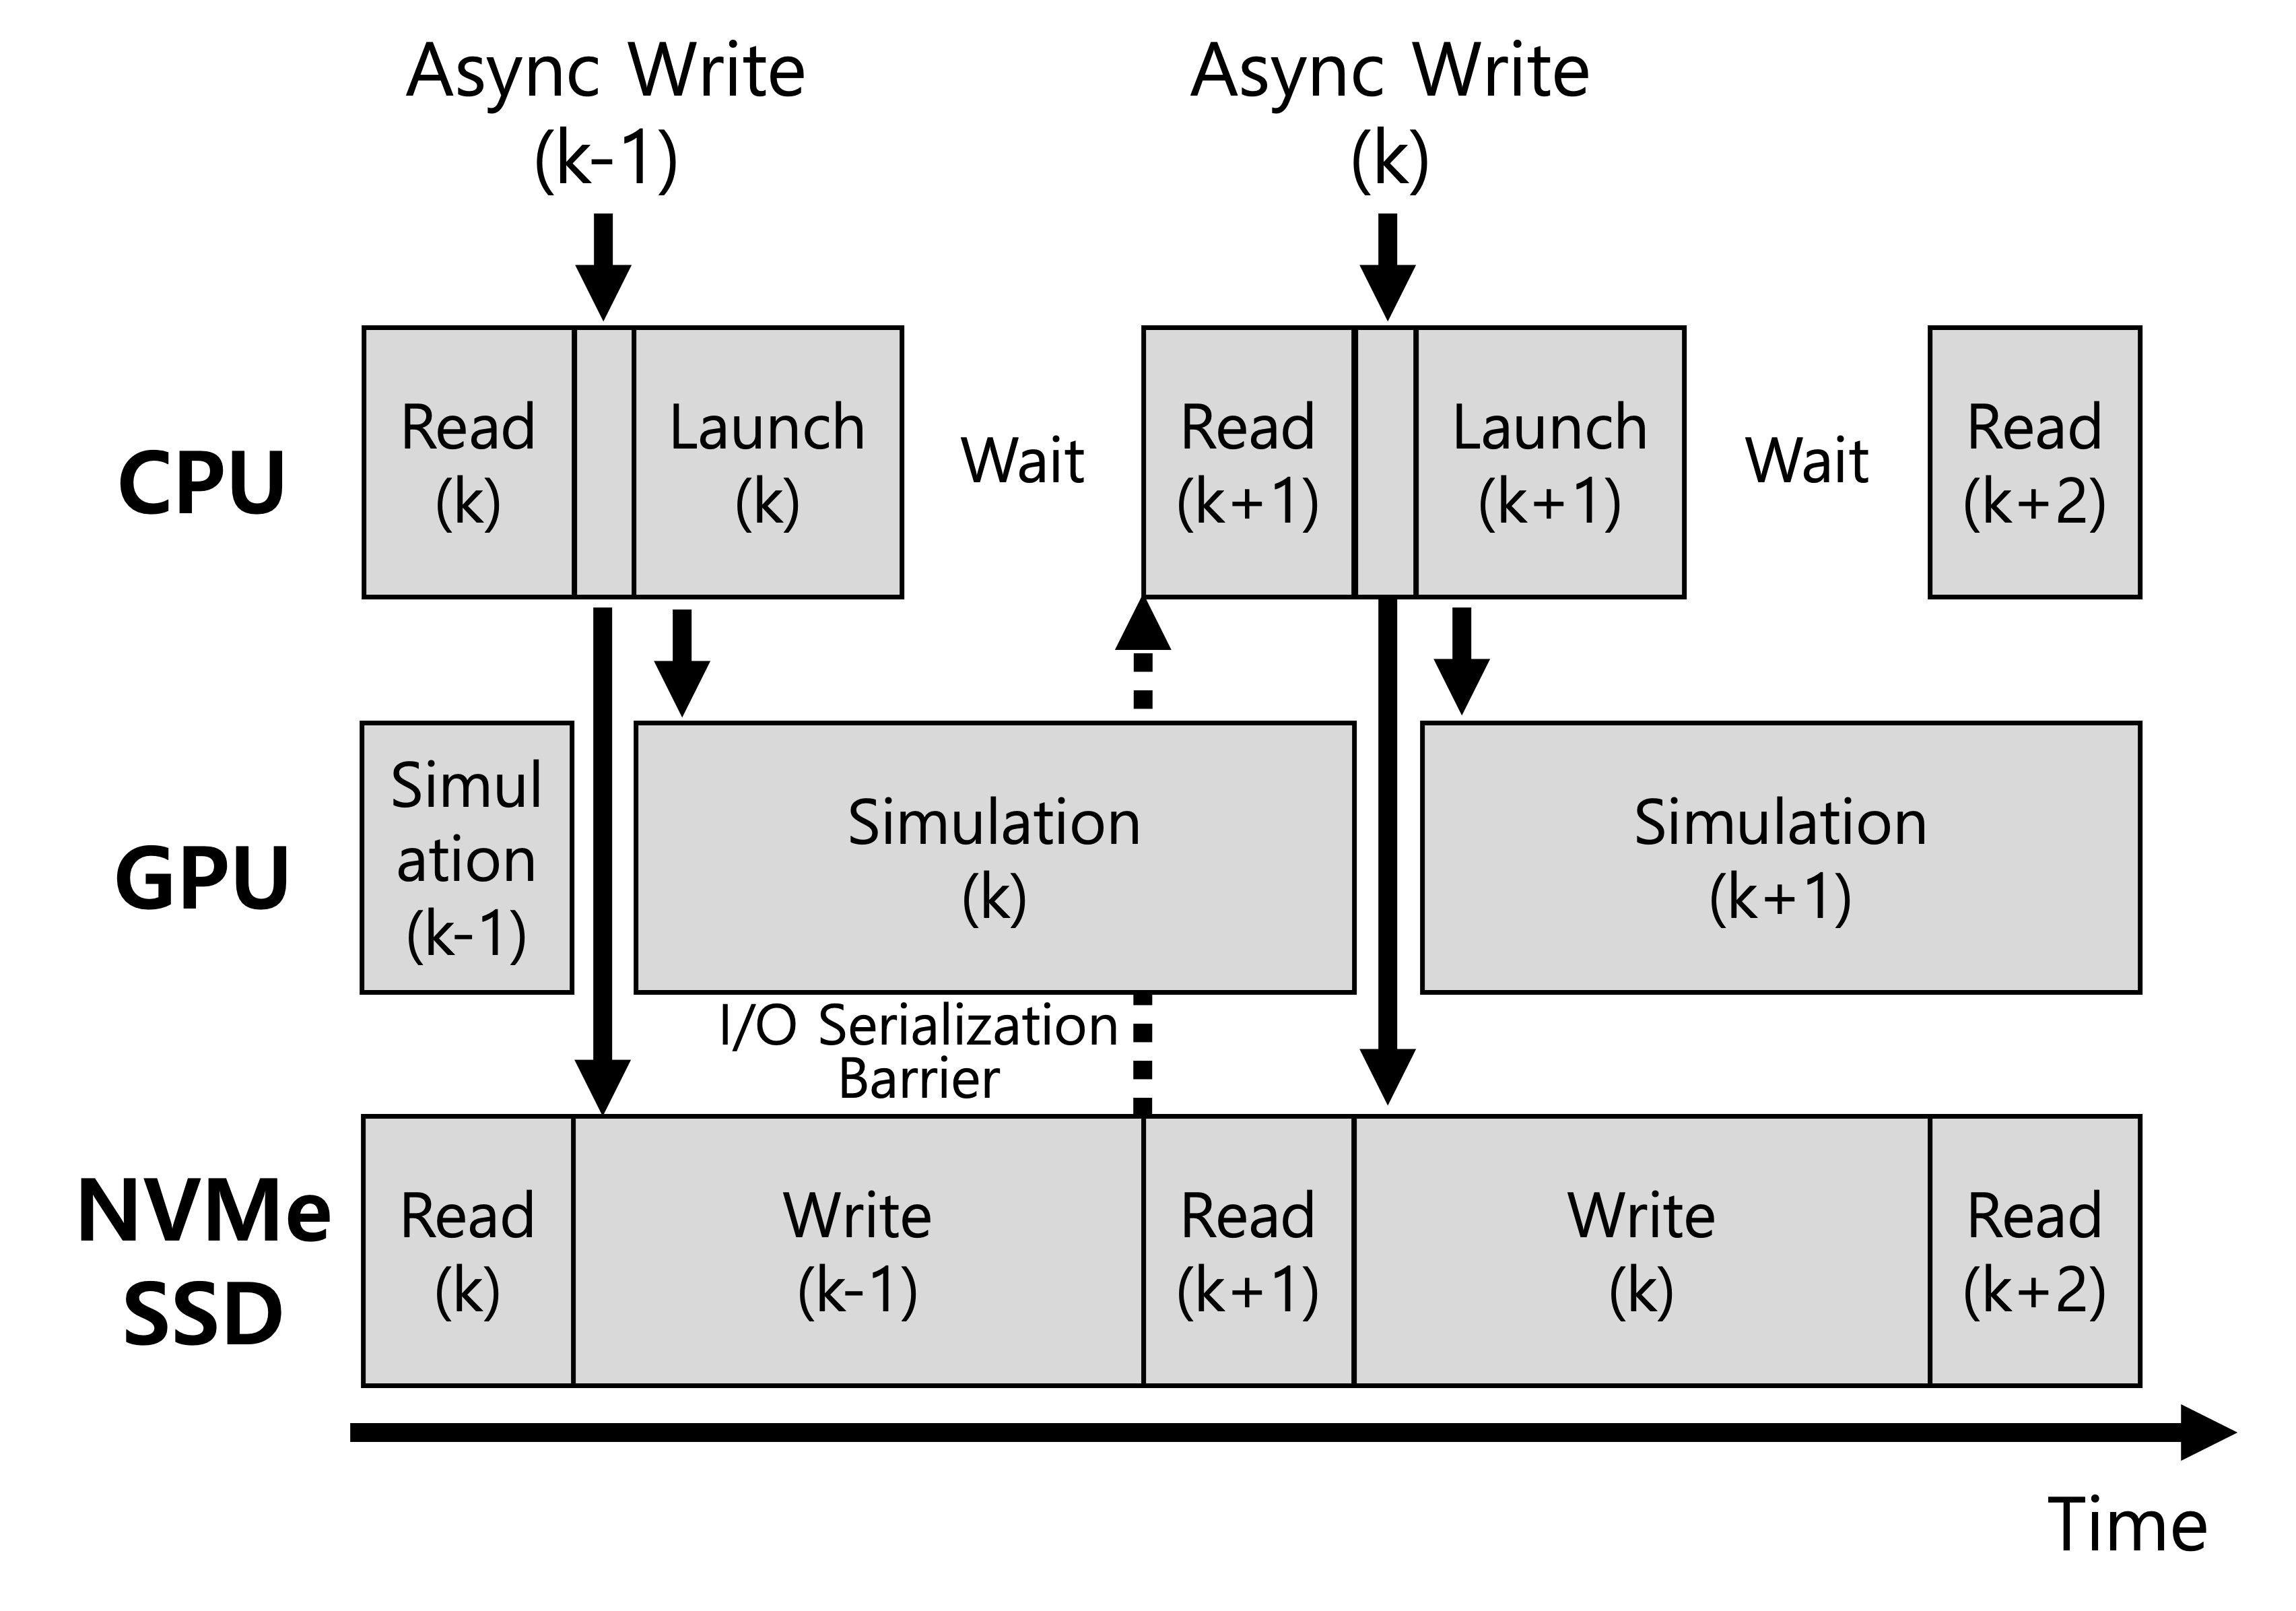
\includegraphics[width=0.85\columnwidth]{Figures/edge_design3.3.png}
    \caption{Execution timeline of the asynchronous pipeline. The dotted line marks the I/O serialization barrier.}
    \vspace{-.2cm}
    \label{design_3.3}
\end{figure}


\begin{enumerate}
\item \textbf{I/O Serialization Barrier:} To avoid bidirectional I/O contention, the CPU halts at a barrier until the background \texttt{pwrite} of an earlier chunk (e.g., $k-2$) completes. This stalling prevents the OS block layer from mixing read/write queues and avoids triggering NVMe garbage collection that delays the subsequent read.
\item \textbf{Synchronous Read:} After clearing the barrier, \EdgeQuantum issues a synchronous \texttt{pread} to load chunk $k$ directly into the UVM ring buffer at sequential read bandwidth.
\item \textbf{Asynchronous Write:} After the read, the framework dispatches a background thread to asynchronously write the previously computed chunk ($k-1$) back to storage.
\item \textbf{GPU Compute Overlap:} Concurrently with the background write, \textit{GPU Compute Engine} executes gate kernels on chunk $k$. Because the Jetson SoC has independent memory and NVMe controllers, computation overlaps with the storage write. This hardware-level separation ensures CPU-intensive I/O and GPU-intensive kernels operate without interference.
\end{enumerate}
By serializing the I/O path and overlapping GPU execution, \EdgeQuantum hides write latency without causing bandwidth contention. 

\noindent\textbf{Cross-Chunk Gate Handling.} Local gates act on amplitudes within a single chunk and are processed within one UVM ring buffer ($q < \log_2(\text{chunk size})$). In contrast, gates targeting qubits beyond the chunk boundary couple amplitudes residing in different chunks, which must be co-resident in memory before invocation. For gates spanning the chunk boundary ($q \geq \log_2(\text{chunk size})$), \EdgeQuantum streams the chunk pair $(c, c \oplus 2^{q-\log_2(\text{chunk size})})$ into two adjacent UVM ring buffers and invokes \textit{cuStateVec} on the paired amplitudes. This pair-wise handling extends to two-global-qubit gates by occupying four ring buffers, matching the 4-buffer depth. Although cross-chunk gates double the per-gate I/O, the asynchronous pipeline overlaps the additional read with GPU compute on the prior pair, preserving throughput characteristics of the local-gate case. Thus, the 4-buffer choice supports both the asynchronous pipeline and cross-chunk gate handling without requiring additional buffers.





\subsection{LZ4 Ping-Pong Compression}
\label{design_compression}
\begin{algorithm}[t]
\caption{Dynamic Ping-Pong Compression Strategy}
\scriptsize
\label{alg:pingpong}
\begin{algorithmic}[1]
\Require Gate Layer $L$, Total Chunks $M$, Truncation Depth $T$
\Ensure Compressed state vector is updated for Layer $L+1$

\State $OffsetOut \gets 0$
\If{$L \bmod 2 = 0$} \Comment{Swap files each layer}
    \State $FileIn, FileOut \gets$ FileA, FileB
    \State $IdxIn, IdxOut \gets$ IndexA, IndexB
\Else
    \State $FileIn, FileOut \gets$ FileB, FileA
    \State $IdxIn, IdxOut \gets$ IndexB, IndexA
\EndIf

\For{$c = 0$ \textbf{to} $M-1$}
    \State $OffsetIn \gets IdxIn[c]$ \Comment{Variable-size read}
    \State $SizeIn \gets IdxIn[c+1] - OffsetIn$
    \State $CompBuf \gets$ \textsc{AsyncRead}$(FileIn, OffsetIn, SizeIn)$
    \State $ShufBuf \gets$ \textsc{LZ4Decompress}$(CompBuf)$ \Comment{Decompress shuffled chunk}
    \State $UVMBuf \gets$ \textsc{ByteUnshuffle}$(ShufBuf)$ \Comment{Restore interleaved float32}
    \State \textsc{GPUCompute}$(UVMBuf)$ \Comment{Apply gates (cross-chunk uses chunk pair)}
    \State \textsc{MantissaTruncate}$(UVMBuf, T)$ \Comment{Zero lower $(23-T)$ mantissa bits}
    \State $ShufBuf \gets$ \textsc{ByteShuffle}$(UVMBuf)$ \Comment{Group same-position bytes}
    \State $SizeOut \gets$ \textsc{LZ4Compress}$(ShufBuf, CompBuf)$ 
    \State \textsc{AsyncWrite}$(FileOut, CompBuf, OffsetOut, SizeOut)$ 
    \State $IdxOut[c] \gets OffsetOut$ \Comment{Update index}
    \State $OffsetOut \gets OffsetOut + SizeOut$
\EndFor
\State $IdxOut[M] \gets OffsetOut$ \Comment{Record total size}

\end{algorithmic}
\end{algorithm}
 

For quantum simulations where the logical state vector exceeds NVMe capacity (e.g., $N \ge 36$ qubits requires $\ge 512$~GB), raw storage becomes a bottleneck. To extend simulation beyond storage limits, \EdgeQuantum integrates a three-stage compression layer combining mantissa truncation, byte shuffle, and LZ4 for low-overhead structure-aware float32 compression. This layer reduces I/O volume by trading CPU cycles for compression overhead. However, gate operations modify the state vector, changing chunk entropy and producing unpredictable compressed sizes. This makes in-place updates infeasible and causes entropy-driven fragmentation.

To address this fragmentation, we design a dynamic ping-pong strategy detailed in Algorithm~\ref{alg:pingpong}. The strategy swaps two backing files, \textit{File A} and \textit{File B}, at the start of each gate layer \textbf{(Lines 2-7)} to enforce atomic updates. During the simulation loop \textbf{(Lines 8-20)}, the framework executes a compressed pipeline for each chunk $c$. First, \EdgeQuantum retrieves the variable-sized compressed chunk via $IdxIn$, decompresses, and reverts the byte shuffle to restore the float32 layout in the UVM ring buffer \textbf{(Lines 9-13)}. Next, \textit{GPU Compute Engine} applies gates to the UVM ring buffer, overlapping with I/O of adjacent chunks \textbf{(Line 14)}. Then, the framework truncates the lower $(23-T)$ mantissa bits, applies byte shuffle to same-position bytes across amplitudes, re-compresses, and appends to the sink file \textbf{(Lines 15-18)}. Finally, the byte offset is recorded in $IdxOut$ for the next gate layer \textbf{(Lines 19-20)}. This append-only strategy avoids file fragmentation and preserves sequential write performance. This dual-file swap enables \EdgeQuantum to simulate a 39-qubit sparse state vector with a 4~TB logical footprint on a 500~GB SSD by reducing the on-disk footprint to approximately 32~GB through up to 255$\times$ per-file compression. The achievable qubit count depends on the per-circuit compression ratio. Circuits with lower compression are supported up to 36 qubits within 500~GB. We adopt $T=8$ in our evaluation, balancing fidelity ($F \geq 0.99$) and compression ratio across the six benchmark circuits (Section~\ref{sec:eval}).


\subsection{\EdgeQuantum Implementation}\label{design_impl}
We implement \EdgeQuantum in C++17 and CUDA 11.4. The  1,350-line codebase is built on four core mechanisms: \texttt{cudaMemAttachHost}-based UVM visibility control for zero-copy UMA handover, \texttt{O\_DIRECT} enabled \texttt{pread}/\texttt{pwrite} for kernel page cache bypass, a multi-threaded asynchronous pipeline for overlapping serialized I/O with GPU compute, and mantissa-truncated LZ4 ping-pong compression for variable-size storage updates.
While optimized for the NVIDIA Jetson Orin Nano, \EdgeQuantum adheres to standard POSIX and CUDA Driver APIs, ensuring portability to other Tegra-based SoC architectures.
\EdgeQuantum provides a C++ API for integration into higher-level quantum simulation frameworks.
%For validation (Section~\ref{sec:eval}), \EdgeQuantum utilizes \textit{cuStateVec} backend for core quantum operations, isolating the performance gains of our tiered memory architecture from underlying compute-engine optimizations.
The source code is publicly available at \url{https://github.com/EdgeQuantum-public/EdgeQuantum}.
\section{Evaluation}
\label{sec:eval}

\subsection{Evaluation Setup}\label{setup} 

\noindent\textbf{Hardware Specification.} We evaluate \EdgeQuantum on the NVIDIA Jetson Orin Nano Developer Kit (8 GB), a representative resource-constrained edge device. The device features an ARM Cortex-A78AE CPU and an NVIDIA Ampere architecture GPU with 1,024 CUDA cores, sharing 8 GB of LPDDR5 unified memory between the CPU and GPU. For storage, we utilize a 500~GB SK hynix PC801 NVMe SSD, providing approximately 1.38~GB/s sequential read and 1.0~GB/s sequential write throughput on the Jetson platform (Section~\ref{back2}). The entire platform operates under a strict 15 W power envelope. 

\noindent\textbf{Baselines.} We compare \EdgeQuantum against three baselines that share the same \textit{cuStateVec} backend for gate execution, isolating the impact of memory and I/O architecture from differences in compute engines. Both \textit{cuQuantum} variants fail to execute on the Jetson 8 GB DRAM at 29 qubits and beyond (Section~\ref{back1}). \textit{cuQuantum (Native)} represents in-memory GPU execution that allocates the full state vector in VRAM. The state vector and CUDA workspace exceed physical capacity and trigger an OOM allocation failure. \textit{cuQuantum (UVM)} extends \textit{cuQuantum} with managed memory. Managed allocations beyond physical DRAM fall back to OS-native swapping that thrashes in the random I/O regime characterized in Section~\ref{back2}. We therefore exclude both from the tiered-regime comparison. \textit{BMQSim-like} is a baseline we implement to isolate the contribution of our 4-buffer pipeline and UVM zero-copy path. It performs out-of-core execution by staging chunks through standard \texttt{cudaMemcpy} with blocking I/O. This follows the design pattern of server-grade tiered simulators such as \textit{BMQSim}. We construct this baseline because BMQSim's build requires server-grade discrete GPUs and PCIe topologies absent from the Jetson SoC.
%For compression evaluation in Section~\ref{sec:extreme_scale}, we additionally compare against \textit{\EdgeQuantum (w/o LZ4)}, an ablation that disables ping-pong compression while retaining the asynchronous pipeline, isolating the contribution of the compression layer to capacity expansion. 

\noindent\textbf{Methodology.} We evaluate \EdgeQuantum using six representative quantum circuits at depth 5 across qubit counts from 30Q (8\,GB) to 39Q (4\,TB): Quantum Volume (QV), Variational Quantum Classifier (VQC), Quantum Support Vector Machine (QSVM), Random circuits, GHZ states, and Variational Quantum Eigensolver (VQE). The qubit range covers two regimes: the tiered-memory regime (30Q-34Q), where the state vector exceeds the 8\,GB DRAM but fits within the 500\,GB SSD, and the compression-required regime (35Q-39Q), where the state vector exceeds SSD capacity and existing simulators fail.


\subsection{Tiered Performance Analysis: 30-34 Qubits}\label{4.2}


\begin{comment}
\begin{table}[t]
\centering
\caption{Simulation time comparison (in seconds) between BMQSim-like (Block) and \EdgeQuantum (Async) for Depth=5.}
\setlength{\tabcolsep}{3pt} % 컬럼 간격 축소
\resizebox{\columnwidth}{!}{%
\begin{tabular}{|l|rr|rr|rr|rr|rr|rr|}
\hline
\textbf{Circuit} & \multicolumn{2}{c|}{\textbf{29Q (4\,GB)}} & \multicolumn{2}{c|}{\textbf{30Q (8\,GB)}} & \multicolumn{2}{c|}{\textbf{31Q (16\,GB)}} & \multicolumn{2}{c|}{\textbf{32Q (32\,GB)}} & \multicolumn{2}{c|}{\textbf{33Q (64\,GB)}} & \multicolumn{2}{c|}{\textbf{34Q (128\,GB)}} \\
 & \multicolumn{1}{c}{Blk} & \multicolumn{1}{c|}{\textbf{EdgeQ}} & \multicolumn{1}{c}{Blk} & \multicolumn{1}{c|}{\textbf{EdgeQ}} & \multicolumn{1}{c}{Blk} & \multicolumn{1}{c|}{\textbf{EdgeQ}} & \multicolumn{1}{c}{Blk} & \multicolumn{1}{c|}{\textbf{EdgeQ}} & \multicolumn{1}{c}{Blk} & \multicolumn{1}{c|}{\textbf{EdgeQ}} & \multicolumn{1}{c}{Blk} & \multicolumn{1}{c|}{\textbf{EdgeQ}} \\
\hline
QV & 29.0 & \textbf{24.6} & 57.7 & \textbf{48.5} & 207.6 & \textbf{171.3} & 450.4 & \textbf{352.9} & 920.8 & \textbf{727.1} & 1853.8 & \textbf{1462.6} \\
VQC & 42.4 & \textbf{38.4} & 95.2 & \textbf{76.9} & 254.7 & \textbf{175.6} & 514.8 & \textbf{361.7} & 1017.9 & \textbf{756.8} & 2069.0 & \textbf{1483.8} \\
QSVM & 16.9 & \textbf{15.5} & 33.9 & \textbf{30.8} & 102.2 & \textbf{70.4} & 203.3 & \textbf{144.7} & 430.7 & \textbf{291.4} & 849.7 & \textbf{593.1} \\
Random & 33.5 & \textbf{29.0} & 67.0 & \textbf{57.8} & 233.9 & \textbf{169.9} & 484.7 & \textbf{357.2} & 974.9 & \textbf{722.7} & 1963.5 & \textbf{1463.9} \\
GHZ & 5.2 & \textbf{4.3} & 10.4 & \textbf{8.6} & 40.8 & \textbf{33.5} & 85.4 & \textbf{70.4} & 173.5 & \textbf{143.5} & 351.1 & \textbf{290.2} \\
VQE & 42.4 & \textbf{38.3} & 84.7 & \textbf{76.9} & 259.0 & \textbf{176.9} & 509.5 & \textbf{361.0} & 1027.9 & \textbf{738.1} & 2050.3 & \textbf{1473.9} \\
\hline
\end{tabular}%
}
\label{tab:main_results}
\end{table}    
\end{comment}

\noindent\textbf{Speedup Across Qubit Scale.} Table~\ref{tab:main_results} compares per-circuit simulation time of \textit{BMQSim-like} baseline and \EdgeQuantum at depth 5 across qubit counts spanning 30Q (8\,GB) to 34Q (128\,GB). \EdgeQuantum consistently outperforms \textit{BMQSim-like} baseline across all configurations. At 30Q (8\,GB), where the chunk count is small and I/O contention is least stressed, the speedup ranges from 1.10$\times$ (QSVM, VQE) to 1.24$\times$ (VQC). As the workload grows to 31--34Q (16--128\,GB), the per-layer I/O volume doubles with each additional qubit and the asynchronous pipeline benefit stabilizes. Speedups widen to 1.21$\times$-1.48$\times$, peaking at 1.48$\times$ for QSVM at 33Q. For VQC at 34Q (128\,GB state vector), \EdgeQuantum saves over nine minutes of execution time (2069.0s$\rightarrow$1483.8s, 1.39$\times$). This trend confirms that the 4-buffer asynchronous pipeline masks NVMe write latency more effectively as cumulative I/O volume grows.

\noindent\textbf{Circuit-Level Behavior.} The speedup magnitude depends on each circuit's gate density, which determines the GPU compute window available to overlap with background writes. Compute-dense circuits (VQC, VQE, Random) show the largest gains (1.34$\times$ to 1.46$\times$ at 31 to 34Q). Their longer gate kernels offer time to hide the 256ms write latency. In contrast, GHZ applies very few gates per layer and shows a stable but lower speedup of $\sim$1.21$\times$ across all qubit counts. The limited compute window leaves less room for overlap. \EdgeQuantum still outperforms blocking I/O by isolating read and write traffic on the NVMe controller, showing that I/O serialization provides a baseline benefit independent of circuit compute density.

\begin{table}[t]
\centering
\caption{Simulation time comparison (in seconds) between \textit{BMQSim-like} (Block) and \EdgeQuantum (Async) without compression (Depth=5).}
\setlength{\tabcolsep}{3pt}
\resizebox{\columnwidth}{!}{%
\begin{tabular}{|l|rr|rr|rr|rr|rr|}
\hline
\textbf{Circuit} & \multicolumn{2}{c|}{\textbf{30Q (8\,GB)}} & \multicolumn{2}{c|}{\textbf{31Q (16\,GB)}} & \multicolumn{2}{c|}{\textbf{32Q (32\,GB)}} & \multicolumn{2}{c|}{\textbf{33Q (64\,GB)}} & \multicolumn{2}{c|}{\textbf{34Q (128\,GB)}} \\
 & \multicolumn{1}{c}{Blk} & \multicolumn{1}{c|}{\textbf{EdgeQ}} & \multicolumn{1}{c}{Blk} & \multicolumn{1}{c|}{\textbf{EdgeQ}} & \multicolumn{1}{c}{Blk} & \multicolumn{1}{c|}{\textbf{EdgeQ}} & \multicolumn{1}{c}{Blk} & \multicolumn{1}{c|}{\textbf{EdgeQ}} & \multicolumn{1}{c}{Blk} & \multicolumn{1}{c|}{\textbf{EdgeQ}} \\
\hline
QV & 57.7 & \textbf{48.5} & 207.6 & \textbf{171.3} & 450.4 & \textbf{352.9} & 920.8 & \textbf{727.1} & 1853.8 & \textbf{1462.6} \\
VQC & 95.2 & \textbf{76.9} & 254.7 & \textbf{175.6} & 514.8 & \textbf{361.7} & 1017.9 & \textbf{756.8} & 2069.0 & \textbf{1483.8} \\
QSVM & 33.9 & \textbf{30.8} & 102.2 & \textbf{70.4} & 203.3 & \textbf{144.7} & 430.7 & \textbf{291.4} & 849.7 & \textbf{593.1} \\
Random & 67.0 & \textbf{57.8} & 233.9 & \textbf{169.9} & 484.7 & \textbf{357.2} & 974.9 & \textbf{722.7} & 1963.5 & \textbf{1463.9} \\
GHZ & 10.4 & \textbf{8.6} & 40.8 & \textbf{33.5} & 85.4 & \textbf{70.4} & 173.5 & \textbf{143.5} & 351.1 & \textbf{290.2} \\
VQE & 84.7 & \textbf{76.9} & 259.0 & \textbf{176.9} & 509.5 & \textbf{361.0} & 1027.9 & \textbf{738.1} & 2050.3 & \textbf{1473.9} \\
\hline
\end{tabular}%
}
\label{tab:main_results}
\end{table}


\subsection{I/O Breakdown without Compression}

\begin{table*}[t]
\centering
\tiny
\caption{I/O Breakdown (seconds) and Speedup from 32 to 34 Qubits.}
\resizebox{\textwidth}{!}{%
\begin{tabular}{|c|c|rrrr|rrrr|r|}
\hline
\multirow{2}{*}{\textbf{Qubits}} & \multirow{2}{*}{\textbf{Circuit}} & \multicolumn{4}{c|}{\textbf{Baseline (Block I/O + cudaMemcpy)}} & \multicolumn{4}{c|}{\textbf{\EdgeQuantum (Async UVM Zero-copy)}} & \multirow{2}{*}{\textbf{Speedup}} \\
\cline{3-10}
 & & \textbf{Read} & \textbf{Comp} & \textbf{Write} & \textbf{Total} & \textbf{Read} & \textbf{Comp} & \textbf{Write} & \textbf{Total} & \\
\hline
\multirow{3}{*}{32Q}
 & VQC & 142.3 & 3.3 & 369.2 & 514.8 & 81.3 & 3.2 & 277.3 & 361.7 & \textbf{1.42$\times$} \\
 & GHZ & 25.2 & 0.5 & 59.7 & 85.4 & 15.6 & 0.5 & 54.4 & 70.4 & \textbf{1.21$\times$} \\
 & VQE & 140.0 & 3.2 & 366.3 & 509.5 & 84.2 & 3.1 & 273.8 & 361.0 & \textbf{1.41$\times$} \\
\hline
\multirow{3}{*}{33Q}
 & VQC & 292.8 & 6.5 & 718.6 & 1017.9 & 177.4 & 6.3 & 573.1 & 756.8 & \textbf{1.35$\times$} \\
 & GHZ & 50.7 & 1.1 & 121.7 & 173.5 & 31.4 & 1.1 & 111.1 & 143.5 & \textbf{1.21$\times$} \\
 & VQE & 286.2 & 6.6 & 735.1 & 1027.9 & 164.5 & 6.1 & 567.6 & 738.1 & \textbf{1.39$\times$} \\
\hline
\multirow{3}{*}{34Q}
 & VQC & 560.7 & 13.4 & 1494.9 & 2069.0 & 328.0 & 12.5 & 1143.3 & 1483.8 & \textbf{1.39$\times$} \\
 & GHZ & 102.7 & 2.2 & 246.3 & 351.1 & 69.7 & 2.0 & 218.5 & 290.2 & \textbf{1.21$\times$} \\
 & VQE & 573.2 & 13.0 & 1464.1 & 2050.3 & 345.8 & 12.0 & 1116.1 & 1473.9 & \textbf{1.39$\times$} \\
\hline
\end{tabular}%
}
\label{tab:io_breakdown}
\end{table*}

Since \EdgeQuantum streams state vector chunks through asynchronous storage I/O while overlapping with GPU computation, the source of its end-to-end speedup must be attributed across distinct phases of the data path. Table~\ref{tab:io_breakdown} decomposes the per-circuit execution time of \textit{BMQSim-like} baseline and \EdgeQuantum into Read, Write, and Compute phases at 32 to 34 qubits.

\noindent\textbf{Read.} Across all configurations, \EdgeQuantum reduces read latency by 1.47$\times$ to 1.75$\times$, with compute-dense circuits at the higher end of the range. For example, at 32Q VQC the read time drops from 142.3s to 81.3s (1.75$\times$). GHZ performs minimal computation and still achieves 1.47$\times$ to 1.62$\times$ read speedup. In contrast, \textit{BMQSim-like} issues concurrent reads and writes that contend within the NVMe controller queue, preventing either direction from sustaining the sequential bandwidth measured in Section~\ref{back2}. By blocking new reads until the preceding write completes (Section~\ref{design_pipeline}), \EdgeQuantum avoids this contention and sustains the 1.38 GB/s sequential read bandwidth.


\noindent\textbf{Write.} The write phase shows a smaller but compute-window-dependent improvement of 1.10$\times$ to 1.34$\times$. Compute-dense circuits (VQC, VQE) achieve 1.25$\times$ to 1.34$\times$ write reductions across 32 to 34Q, with 34Q VQE dropping from 1464.1s to 1116.1s. In contrast, \textit{BMQSim-like} blocks on each \texttt{pwrite}, exposing the full latency. By overlapping background \texttt{pwrite} with GPU compute, \EdgeQuantum masks the 256ms write latency when the compute window is sufficient. GHZ consumes only 0.5 to 2.2s of compute, with insufficient overlap yielding only 1.10$\times$ to 1.13$\times$ reductions. This circuit-dependent behavior validates the compute-overlap design from Section~\ref{design_pipeline}.

\noindent\textbf{Compute.} The compute phase remains nearly identical between the two schemes, differing by at most 10\% and rarely exceeding 1s in absolute terms (e.g., 13.4s vs 12.5s at 34Q VQC). This confirms that the end-to-end speedup originates from the I/O data path rather than the gate-execution path. Both schemes use \textit{cuStateVec} backend, and \EdgeQuantum introduces no additional kernel-level overhead.


\subsection{Storage Efficiency}

\begin{figure}[t]
    \centering
    \begin{subfigure}[b]{0.45\columnwidth}
        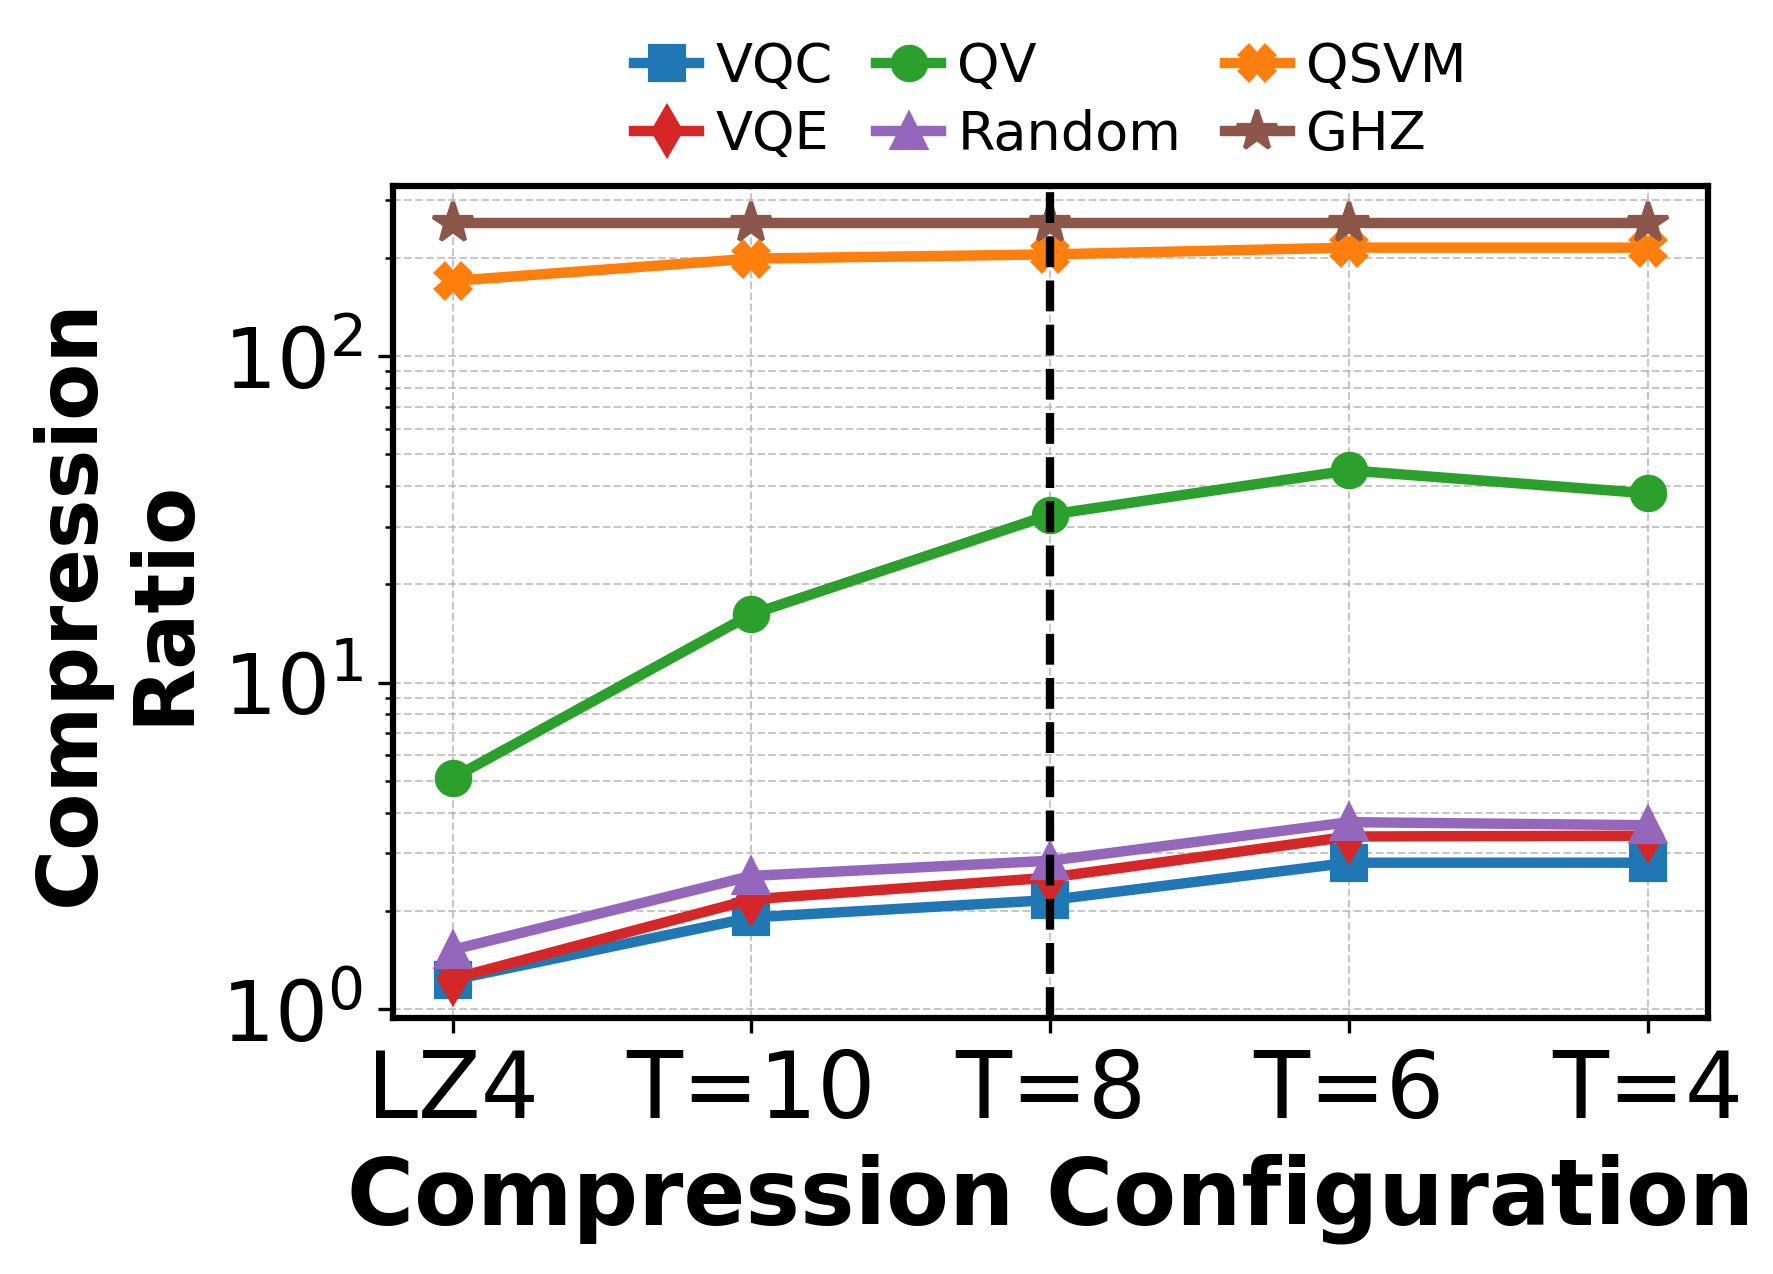
\includegraphics[width=\linewidth]{Figures/compress1.png}
        \caption{Compression ratio across truncation depths.}
        \label{fig:eff_ratio}
    \end{subfigure}\hfill
    \begin{subfigure}[b]{0.54\columnwidth}
        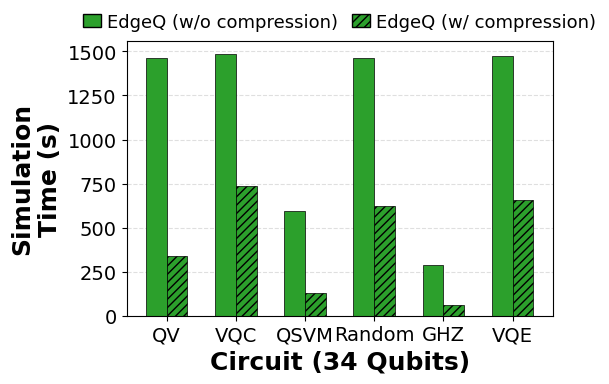
\includegraphics[width=\linewidth]{Figures/compress2.png}
        \caption{Compression speedup at 34 qubits.}
        \label{fig:eff_speedup}
    \end{subfigure}
    \caption{Storage efficiency from mantissa-truncated LZ4 compression.}
    \label{fig:storage_eff}
\end{figure}


Since the 500GB physical NVMe SSD on the Jetson platform cannot accommodate raw state vectors beyond 35 qubits in the dual-file ping-pong layout, \EdgeQuantum uses ping-pong mantissa-truncated LZ4 compression to extend simulation capacity. Figure~\ref{fig:storage_eff} reports two measurements. Figure~\ref{fig:eff_ratio} shows per-circuit compression ratio across the LZ4 baseline and four mantissa truncation depths. Figure~\ref{fig:eff_speedup} shows per-circuit speedup at 34Q, where uncompressed state vectors dominate I/O time.

\noindent\textbf{Compression Ratio Sweep.} Figure~\ref{fig:eff_ratio} compares per-circuit compression ratios across the LZ4 baseline and four mantissa truncation depths. As truncation depth decreases from $T=10$ to $T=8$, the QV ratio expands from 16.2$\times$ to 32.7$\times$, while the VQC ratio scales from 1.91$\times$ to 2.16$\times$. Each truncation depth zeros the lower mantissa bits before LZ4, corresponding to per-file ratios from 2.16$\times$ (VQC) to 255$\times$ (GHZ) at $T=8$ across the six circuits. The byte shuffle groups same-position bytes across amplitudes to expose zero-runs in the truncated lower bytes, yielding ratios above the LZ4-only baseline by up to 6$\times$ for QV. The $T=8$ point reflects the chosen operating depth, whereas $T=6$ further increases the ratio for QV (32.7$\times$$\rightarrow$44.7$\times$) and $T=4$ reduces it (44.7$\times$$\rightarrow$38.0$\times$). Thus, \EdgeQuantum fits a 39-qubit GHZ simulation within 32GB of NVMe storage at $T=8$, whereas dense circuits achieve per-file compression of 2.16$\times$-2.85$\times$ that supports up to 36 qubits within the 500GB capacity.


\noindent\textbf{Performance Benefit.} Figure~\ref{fig:eff_speedup} compares per-circuit simulation time of \EdgeQuantum with and without mantissa-truncated LZ4 compression at 34Q, isolating the compression speedup from capacity necessity since the raw state vector still fits the 500GB SSD without compression. Compression yields a 1.73$\times$-4.59$\times$ speedup across the six circuit types, with the largest gain on GHZ (290.2s $\rightarrow$ 63.3s, 4.59$\times$) and the smallest on VQC (1483.8s $\rightarrow$ 858.2s, 1.73$\times$). This range arises because the per-circuit compression ratio determines I/O reduction between UVM and NVMe, and high-ratio circuits (GHZ, QSVM, QV) transition into a regime dominated by compression and decompression overhead while dense circuits (VQC, Random, VQE) remain partially I/O-bound. At 34Q, all circuits start heavily I/O-bound regardless of compute density, so compression delivers speedup proportional to the I/O reduction it provides. The asynchronous pipeline alone capped GHZ at 1.21$\times$ (Section~\ref{4.2}) because its narrow compute window limited write-latency overlap. Compression bypasses this compute-window dependence by reducing I/O volume directly, so GHZ achieves a 4.59$\times$ speedup that matches the high-ratio circuits (QSVM 4.57$\times$, QV 4.18$\times$) and exceeds the dense circuits (1.73$\times$-2.04$\times$).




\subsection{Extreme Scalability: 35–39 Qubits}


\begin{table}[t]
\centering
\scriptsize
\caption{Extreme-scale simulation times (seconds) for \EdgeQuantum with mantissa-truncated LZ4 compression at $T=8$ (Depth=5). Dash indicates configurations that exceed the 500GB SSD capacity in the dual-file ping-pong layout.}
\resizebox{\columnwidth}{!}{%
\begin{tabular}{|l|r|r|r|r|r|}
\hline
\textbf{Circuit} & \textbf{35Q (256GB)} & \textbf{36Q (512GB)} & \textbf{37Q (1TB)} & \textbf{38Q (2TB)} & \textbf{39Q (4TB)} \\
\hline
GHZ    & 119.10 & 246.77 & 492.53 & 990.21 & 1,980.20 \\
QSVM   & 251.69 & 494.23 & 982.25 & 1,981.10 & 3,974.19 \\
QV     & 650.45 & 1,355.27 & 2,683.68 & 5,445.10 & 10,811.64 \\
\hline
Random & 1,328.69 & 2,739.91 & --- & --- & --- \\
VQE    & 1,486.57 & 2,949.12 & --- & --- & --- \\
VQC    & 1,619.05 & 3,295.61 & --- & --- & --- \\
\hline
\end{tabular}%
}
\label{tab:extreme_results}
\end{table}

Beyond 34 qubits, the logical state vector exceeds the 500GB SSD capacity by up to 8$\times$ (4TB at 39Q). This makes the mantissa-truncated LZ4 ping-pong compression layer mandatory for execution, enabling \EdgeQuantum to operate where alternative simulators fail. Table~\ref{tab:extreme_results} shows the per-circuit simulation times across 35Q (256GB) to 39Q (4TB).

As shown in the table, \EdgeQuantum exhibits stable, near-linear scalability as the state vector doubles at each qubit increment. For high-ratio circuits (GHZ, QSVM, QV), runtime tracks the 16$\times$ data volume growth, increasing 15.8$\times$$-$16.6$\times$ from 119.1s$-$650.5s at 35Q to 1,980.2s$-$10,811.6s at 39Q (e.g., 10,811.6s or $\approx$3.00 hours for QV). Dense circuits stop at 36Q within the 500GB capacity, with Random, VQE, and VQC completing 36Q in 2,739.9s, 2,949.1s, and 3,295.6s, respectively. This near 2$\times$ time growth per qubit confirms that the ping-pong pipeline maintains compression throughput at the 4~TB scale for high-ratio circuits without degradation from queue contention or fragmentation.

This regime is accessible to \EdgeQuantum because of its UMA-optimized compression path. Server-grade simulators such as \textit{BMQSim} apply compression at the GPU level, relying on VRAM to stage and compress data, which is infeasible on edge devices. When the logical state vector reaches or exceeds the 500GB SSD capacity in the ping-pong layout ($\geq$35Q), the raw state cannot be persisted on disk, leaving \textit{BMQSim-like} with no chunks to stage from storage. Even at smaller scales, dedicating GPU cycles to compression contends with quantum gate kernels for the same compute resources. By performing mantissa-truncated LZ4 compression on the CPU during the I/O offloading phase, \EdgeQuantum exploits otherwise idle CPU cores and preserves GPU compute cycles for quantum gate operations. Among the three baselines defined in Section\ref{setup}, \textit{cuQuantum} variants fail at 29Q because of DRAM exhaustion, and \textit{BMQSim-like} cannot start beyond 34Q because of SSD exhaustion, leaving \EdgeQuantum as the only framework to reach the 4TB regime on this 8GB device.

\subsection{I/O Breakdown with Compression}\label{sec:io_breakdown_compressed}

\begin{table}[t]
\centering
\caption{I/O breakdown (seconds) for \EdgeQuantum with mantissa-truncated LZ4 ping-pong compression across 34-36 qubits.}
\setlength{\tabcolsep}{3pt}
\scriptsize
\resizebox{\columnwidth}{!}{%
\begin{tabular}{|c|c|r|r|r|r|r|r|}
\hline
\textbf{Qubits} & \textbf{Circuit} & \textbf{pread} & \textbf{decomp.} & \textbf{compute} & \textbf{compress} & \textbf{pwrite} & \textbf{Total} \\
\hline
\multirow{3}{*}{34Q}
 & VQC & 158.9 & 226.9 & 12.6 & 84.1 & 375.7 & 858.2 \\
 & GHZ & 0.4 & 44.3 & 2.0 & 15.7 & 0.9 & 63.3 \\
 & VQE & 148.9 & 221.3 & 11.8 & 82.1 & 310.1 & 774.2 \\
\hline
\multirow{3}{*}{35Q}
 & VQC & 348.9 & 421.6 & 25.1 & 157.4 & 666.0 & 1619.0 \\
 & GHZ & 0.5 & 83.3 & 4.1 & 29.6 & 1.6 & 119.1 \\
 & VQE & 275.4 & 426.4 & 24.3 & 159.4 & 601.0 & 1486.5 \\
\hline
\multirow{3}{*}{36Q}
 & VQC & 723.5 & 856.7 & 50.9 & 320.9 & 1343.6 & 3295.6 \\
 & GHZ & 1.0 & 172.8 & 8.0 & 61.8 & 3.2 & 246.8 \\
 & VQE & 578.7 & 847.6 & 49.6 & 314.1 & 1159.1 & 2949.1 \\
\hline
\end{tabular}%
}
\label{tab:io_breakdown_compressed}
\end{table}



Table~\ref{tab:io_breakdown_compressed} decomposes the execution time of \EdgeQuantum with mantissa-truncated LZ4 ping-pong compression into physical I/O, CPU compression, and GPU compute phases across 34 to 36 qubits.

\noindent\textbf{Bottleneck Shift for High-Ratio Circuits. }Compression and decompression dominate the total execution time for high-ratio circuits, shifting the primary bottleneck from physical I/O to the CPU. For 34Q GHZ, physical I/O operations (\texttt{pread} and \texttt{pwrite}) account for 1.3s, representing 2.1\% of the 63.3s total execution time. Conversely, CPU-driven LZ4 decompression and compression consume 60.0s, constituting 94.8\% of the total duration. This profile demonstrates that the 255$\times$ data volume reduction eliminates the NVMe bandwidth constraint. The system transitions into a CPU-bound regime where execution time depends primarily on compression throughput, validating the design trade-off introduced in Section~\ref{design_compression}.

\noindent\textbf{Linear Scaling and Task Overlap. }As the logical state vector scales from 34Q to 36Q, the execution phases exhibit stable linear growth without triggering OS-level thrashing or I/O contention. For GHZ, CPU decompression time scales from 44.3s (34Q) to 172.8s (36Q), approximately doubling per qubit increment. Across all scales, GPU compute time remains a small fraction of total runtime, requiring 2.0s to 50.9s per simulation. Because the combined CPU LZ4 phase exceeds GPU compute by over an order of magnitude, the GPU compute window is fully absorbed by the background offloading tasks. This validates the UMA-optimized compression path, which overlaps CPU LZ4 with GPU gate execution on shared DRAM. By utilizing otherwise-idle CPU cores for LZ4 processing, \EdgeQuantum extends simulation capacity while maintaining predictable scaling across both CPU-bound (high-ratio) and I/O-bound (dense) regimes.



\subsection{Impact of Buffer Depth}
Figure~\ref{fig:buffer_impact} shows the impact of UVM buffer count on simulation performance at two contrasting state vector scales: 32Q (32~GB) and 36Q (512~GB). Other parameters, such as chunk size (256~MB) and circuit depth (5), are fixed to isolate the buffer-depth effect. While a single buffer executes sequentially without overlap, increasing the buffer count to 4 yields the best performance at both scales, achieving 1.04$\times$-1.12$\times$ speedup at 32Q and 1.02$\times$-1.08$\times$ speedup at 36Q across all circuits. This confirms that \EdgeQuantum's asynchronous pipeline hides NVMe write latency by overlapping it with GPU computation, as described in Section~\ref{design_pipeline}. However, increasing the buffer count beyond 4 progressively reduces this benefit, and the degradation amplifies as the state vector grows.

At 32Q, where the working set occupies a moderate fraction of physical memory, 6- and 8-buffer configurations remain marginally faster than the 1-buffer baseline but lose the gain achieved at 4 buffers. At 36Q, where the active working set occupies most of the available DRAM, over-allocation pushes the buffer pool beyond the headroom of physical memory, triggering UVM page faults and OS-level thrashing. As a result, the 8-buffer configuration runs approximately 0.7-0.8\% slower than the 1-buffer baseline for QSVM, Random, and GHZ. Thus, the 4-buffer choice in \EdgeQuantum's \textit{Tiered Mode} (Section~\ref{design_pipeline}) provides the highest pipeline benefit with minimal residency cost and remains stable across the 32Q to 36Q scale-up.


\begin{figure}[!t]
    \centering
    \hspace*{0.09\linewidth}
    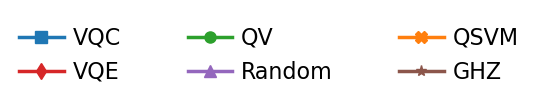
\includegraphics[width=0.6\linewidth]{Figures/lagend_buffers.png}
    \vspace{-.2cm}

    \subfloat[32 Qubits (32\,GB).]{
        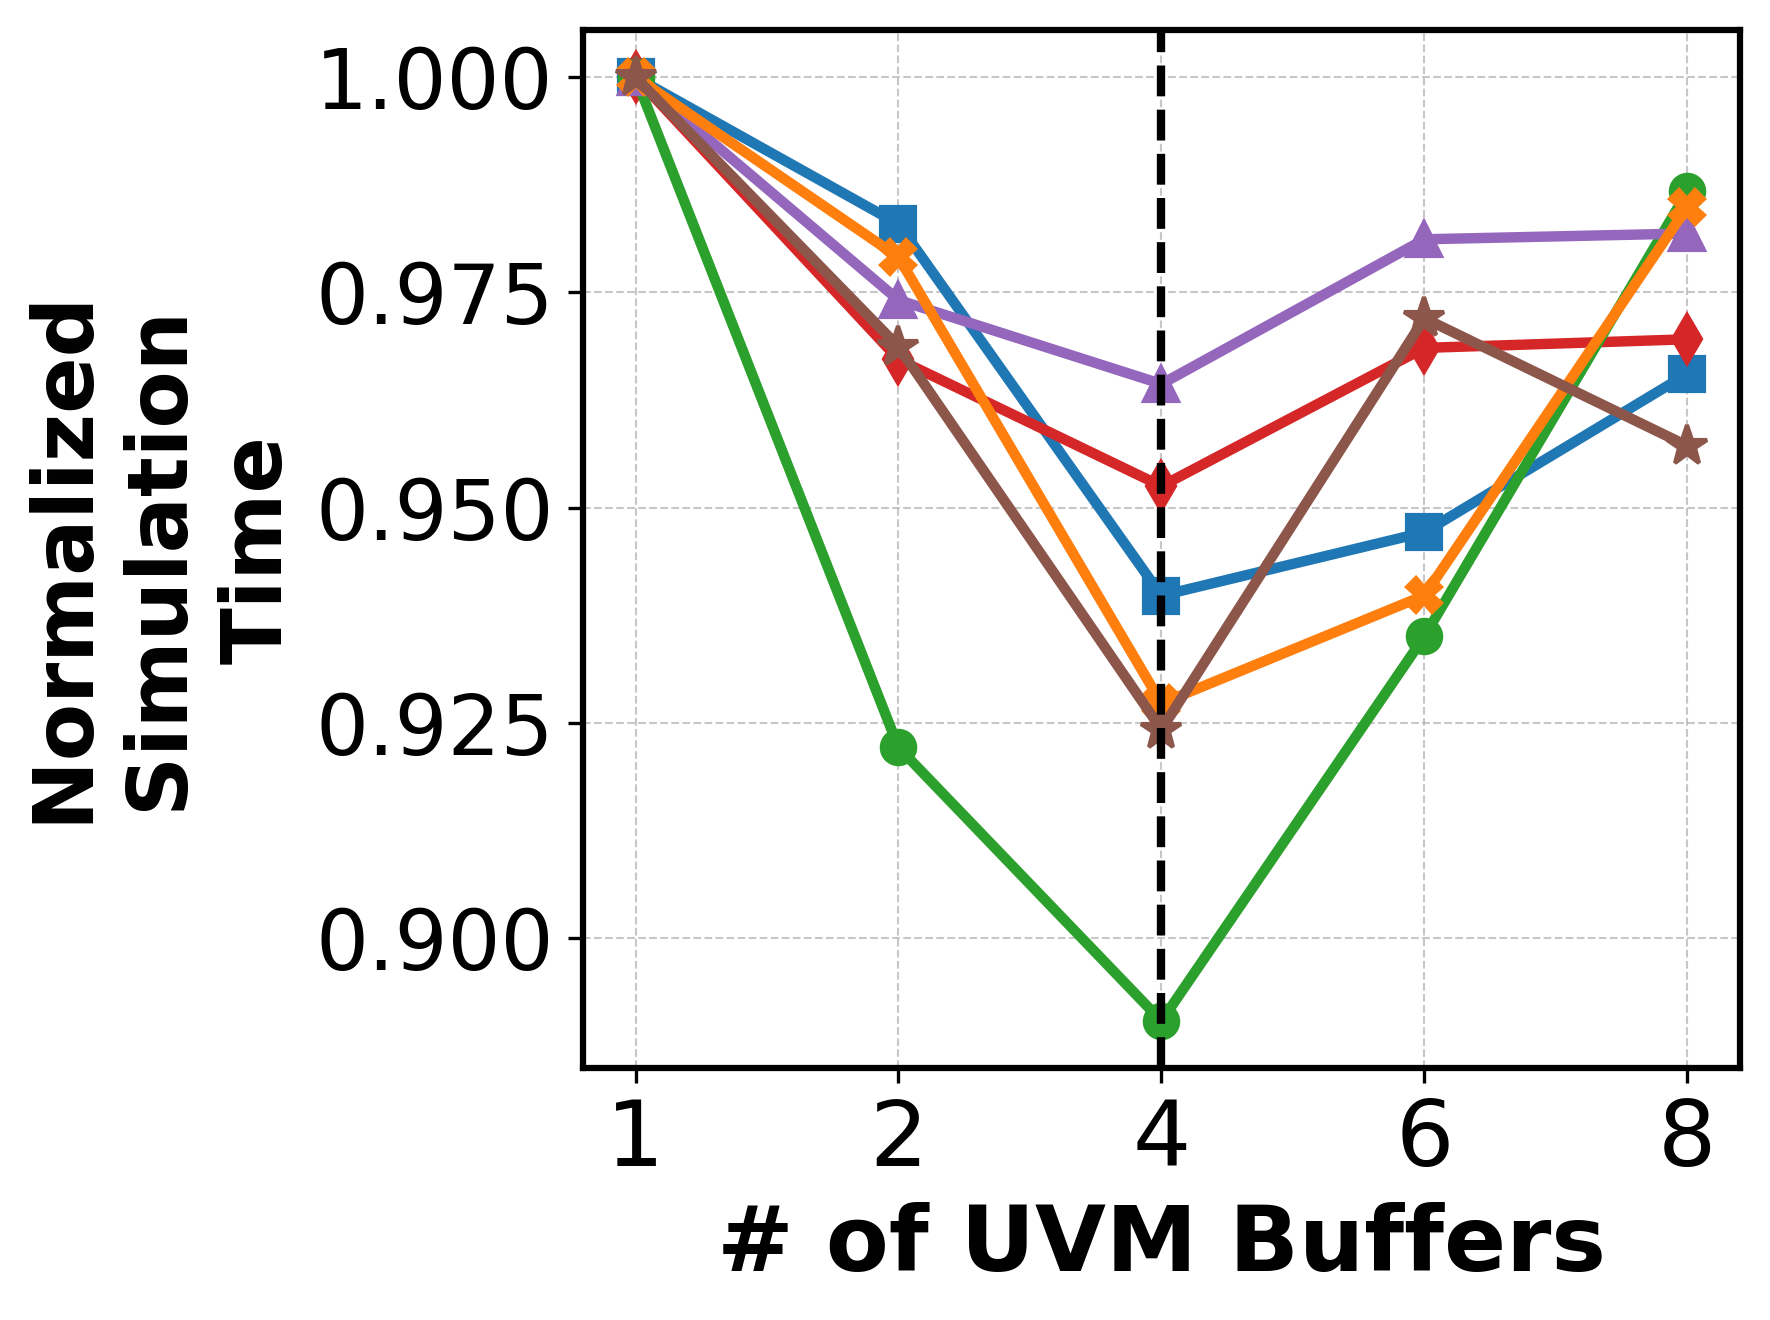
\includegraphics[width=0.46\linewidth]{Figures/32buffer.png}
        \label{fig:buffer_32q}
        \vspace{-.3cm}
    }
    \subfloat[36 Qubits (512\,GB).]{
        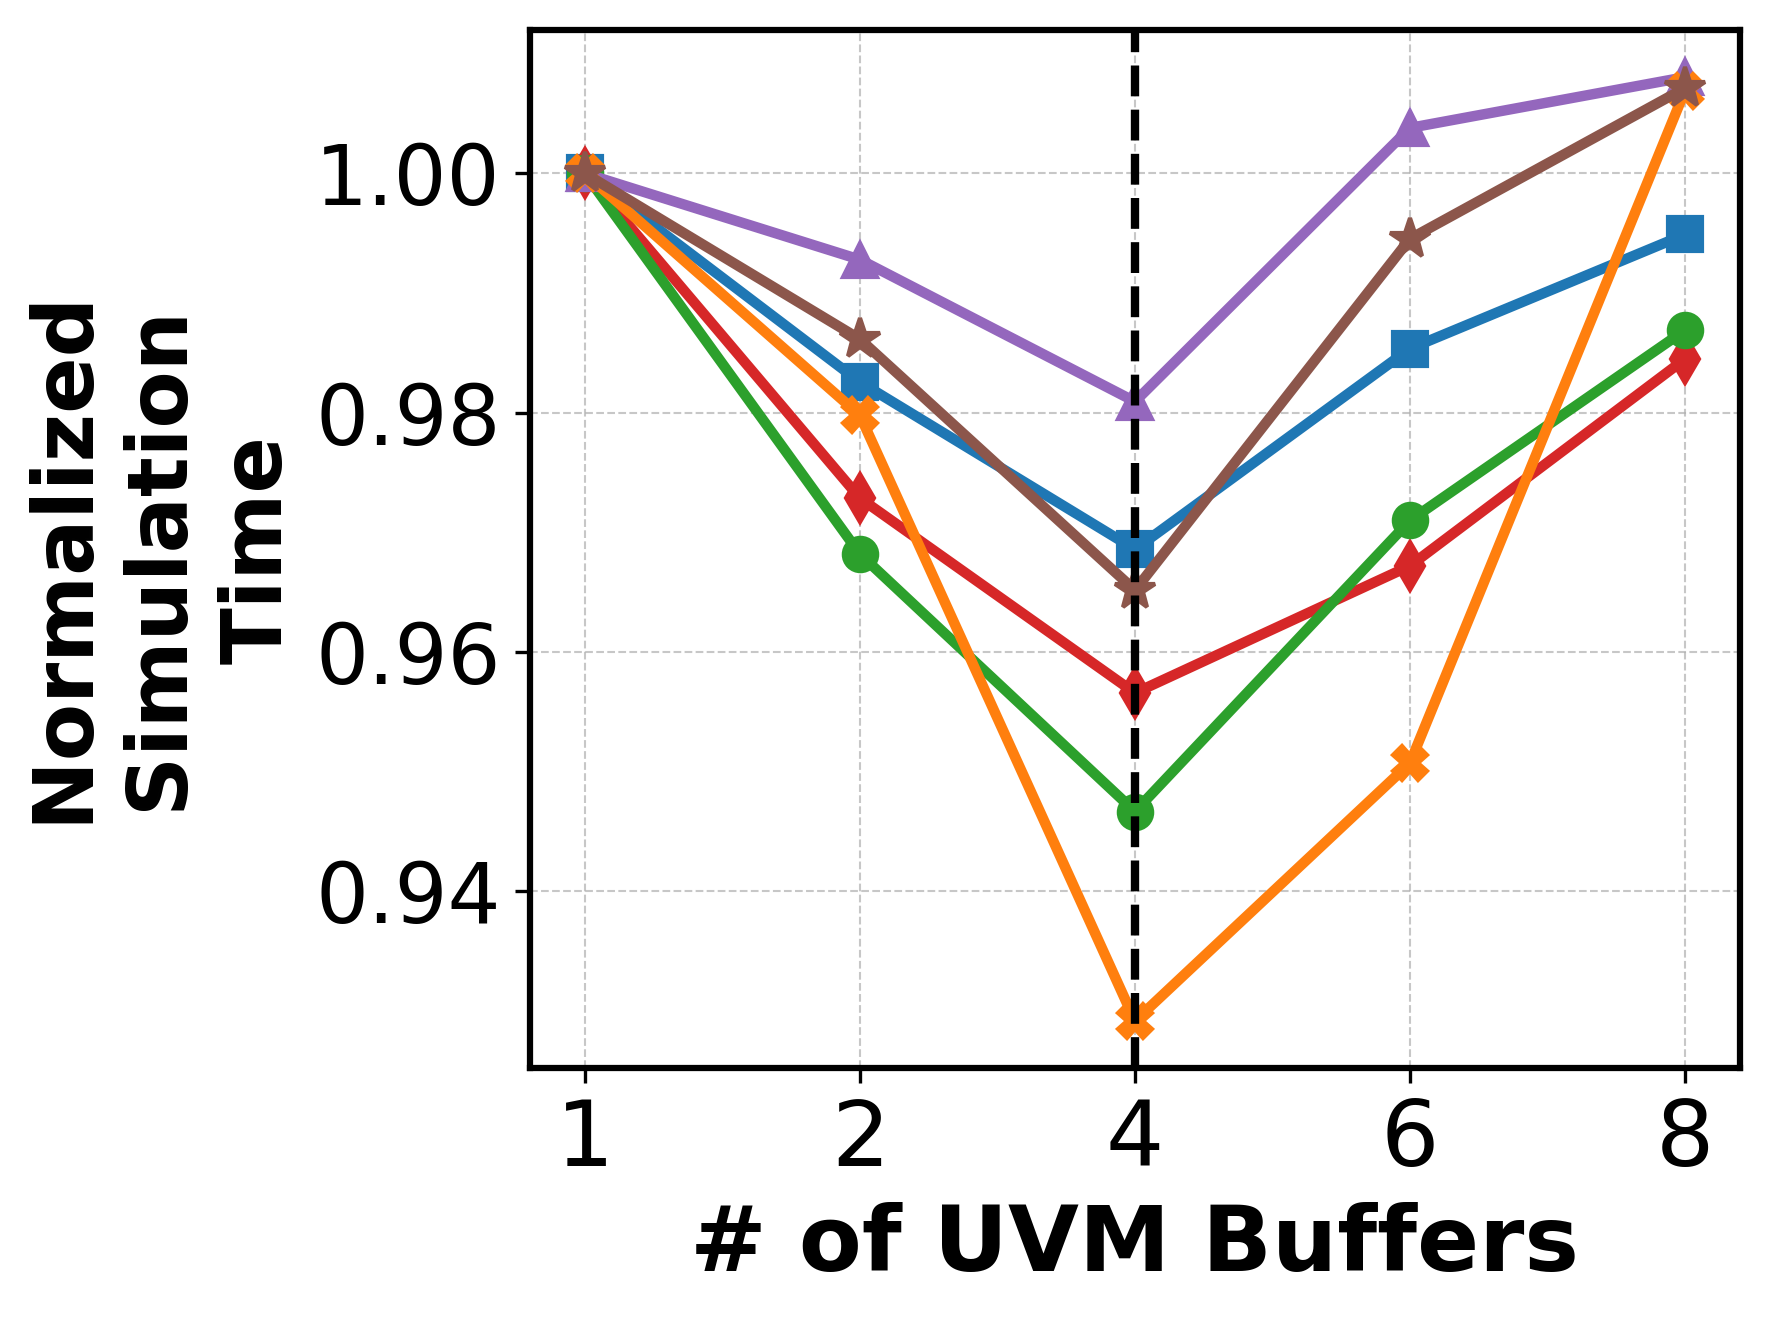
\includegraphics[width=0.46\linewidth]{Figures/36buffer.png}
        \label{fig:buffer_36q}
        \vspace{-.3cm}
    }
    \vspace{-.2cm}
    \caption{Impact of UVM buffer count on simulation time at two state vector scales.}
    \vspace{-.2cm}
    \label{fig:buffer_impact}
\end{figure}


\subsection{Fidelity and Stability}
Since \EdgeQuantum partitions the state vector and relies on frequent I/O, ensuring numerical stability is critical.
We verified the fidelity of the final state vector against small-scale \textit{Cirq} CPU simulations for verifying correctness.

\begin{table}[t]
\centering
\caption{State fidelity $F = |\langle\psi_\text{exact}|\psi_\text{lossy}\rangle|^2$ at depth 5 across truncation depths. Bold column marks the chosen operating depth ($T=8$).}
\label{tab:fidelity}

\setlength{\tabcolsep}{4pt}
\renewcommand{\arraystretch}{1.1}

\footnotesize
\begin{tabular}{c|c|c|c|c}
\hline
\textbf{Circuit} & \textbf{T=10} & \textbf{T=8} & \textbf{T=6} & \textbf{T=4} \\
\hline
GHZ    & 0.9998 & \textbf{0.9998} & 0.9888 & 0.9453 \\
QSVM   & 0.9993 & \textbf{0.9982} & 0.9885 & 0.9553 \\
QV     & 0.9970 & \textbf{0.9919} & 0.9453 & 0.7812 \\
Random & 0.9965 & \textbf{0.9952} & 0.9544 & 0.8213 \\
VQE    & 0.9957 & \textbf{0.9938} & 0.9470 & 0.8114 \\
VQC    & 0.9968 & \textbf{0.9983} & 0.9514 & 0.7900 \\
\hline
\end{tabular}
\end{table}

For all circuits up to 30 qubits (where verification is feasible), Table~\ref{tab:fidelity} reports the measured state fidelity across truncation depths $T \in \{10, 8, 6, 4\}$ at depth 5. At the chosen $T=8$ operating point, fidelity ranges from 0.9919 (QV) to 0.9998 (GHZ), maintaining $F \geq 0.99$ across the six circuits. Lower $T$ values trade fidelity for compression: $T=6$ drops dense circuits to 0.9453--0.9544 and $T=4$ further to 0.78-0.95, while $T=10$ raises all circuits above 0.9957 at the cost of weaker compression (Figure~\ref{fig:eff_ratio}).
The successful completion of 151 benchmark runs without a single crash or I/O error validates the robustness of the 4-buffer pipeline and the UVM management logic.



\section{Related Work}
\label{sec:related}
\noindent\textbf{Optimizing Quantum Circuit Simulation.} Previous studies on quantum circuit simulation utilize massive parallelism in GPUs and distributed clusters for full state vector simulation, distributing the state across aggregated VRAM in leadership-class supercomputers~\cite{10.1145/3771577, haner20175, chen201864}. Other studies propose static compilation and circuit partitioning to reduce communication overhead, maximizing kernel occupancy through precompiled kernels~\cite{xu2024atlas, zhang2021hyquas, li2021sv}. Additionally, tensor network-based approaches reduce memory footprint by decomposing quantum states into interconnected tensors, providing savings for low-entanglement circuits while facing exponential complexity in deep entangled circuits~\cite{burgholzer2022simulation, kim2025swiftn, huang2021efficient, lykov2022tensor}. Our study aligns with these efforts. However, existing server-centric approaches assume abundant memory and high-bandwidth interconnects, failing on edge devices with limited DRAM (e.g., 8~GB). In contrast, \EdgeQuantum's UMA-aware tiered memory architecture partitions the state vector across storage tiers via a UVM zero-copy data path. A 4-buffer ring pipeline and mantissa-truncated LZ4 ping-pong compression extend simulation capacity beyond DRAM.

\noindent\textbf{Memory Expansion and I/O Optimization Strategies.} Previous studies on memory expansion focus on extending simulation capacity by offloading state vectors to high-performance NVMe SSDs in server environments through OS-level demand paging or explicit memory mapping~\cite{park2022snuqs, zhang2025bmqsim}. Other work proposes lossless compression and adaptive encoding to trade CPU cycles for capacity~\cite{zhang2025bmqsim, wu2018memory, wu2019full, song2023efficient}. In the broader context of deep learning, prior studies reduce memory pressure by offloading intermediate feature maps to secondary storage~\cite{7783721, 264816, 10.1145/3630108}. While our study aligns with these techniques, generic strategies fail on edge devices due to SSD asymmetry and UMA constraints. Prior server-centric frameworks target high-end infrastructure and ignore variable-size update constraints on commodity edge storage. \EdgeQuantum's asynchronous I/O strategy serializes reads and writes to avoid NVMe contention, built on a UMA-aware UVM zero-copy data path that eliminates \texttt{cudaMemcpy} staging. A dual-file ping-pong mantissa-truncated LZ4 compression layer extends storage capacity beyond SSD limits.

\begin{comment}
  
\subsection{Optimizing Quantum Circuit Simulation}


There have been many studies that optimize quantum circuit simulation to enhance performance on high-end hardware.
Previous studies focused on utilizing massive parallelism in GPUs and distributed clusters for full state vector simulation.
These approaches accelerate execution and extend scalability by distributing the state vector across aggregated video memory (VRAM) in leadership-class supercomputers.
Other studies have proposed static compilation and circuit partitioning techniques to reduce communication overhead.
These methods analyze quantum circuits in advance to generate optimized execution plans or precompiled kernels, aiming to maximize kernel occupancy and minimize inter-node data transfer.
In addition, tensor network-based approaches have been proposed to reduce the memory footprint by decomposing quantum states into interconnected tensors.
These methods provide significant memory savings for shallow or low-entanglement circuits but face exponential complexity growth when simulating deep circuits with high entanglement.

Our study aligns with these prior efforts in improving the computational efficiency of quantum circuit simulation.
However, \EdgeQuantum aims to democratize quantum simulation by targeting resource-constrained edge devices rather than relying on inaccessible HPC infrastructure.
Existing datacenter-centric approaches such as \textit{ScaleQsim} and \textit{cuQuantum} assume abundant memory resources and high-bandwidth interconnects, which leads to execution failures on embedded devices where physical memory is strictly limited (e.g., 8 GB).
Through a tiered-memory architecture, \EdgeQuantum partitions the state vector across the storage hierarchy rather than across network nodes, and employs a specialized 4-buffer pipeline.
This allows \EdgeQuantum to enable large-scale simulation on commodity hardware without requiring millions of dollars in infrastructure.

\subsection{Memory Expansion and I/O Optimization Strategies}

To address the physical memory bottleneck, several simulation frameworks and system-level optimizations have been proposed to utilize secondary storage or compression.
Previous studies focused on extending simulation capacity by offloading state vectors to high-performance NVMe SSDs in server environments.
These approaches manage the movement of data pages between host memory and storage, often relying on OS-level demand paging or explicit memory mapping (mmap) to support simulations exceeding physical RAM capacity.
Other studies have proposed lossless compression and adaptive error-bounded encoding techniques to reduce memory consumption.
These methods dynamically compress state vectors during simulation, allowing systems to store larger quantum states within limited memory footprints by trading CPU cycles for capacity.
In the broader context of deep learning, approaches such as vDNN and FlashNeuron simplify memory management by offloading intermediate feature maps to backing stores.

These approaches highlight key techniques for improving capacity in data-intensive applications.
Similarly, \EdgeQuantum faces comparable challenges in edge quantum simulation, where the state vector size far exceeds the unified memory capacity of the SoC.
However, applying generic offloading techniques to edge devices is inefficient due to the bandwidth asymmetry of consumer-grade SSDs and the specific constraints of the Unified Memory Architecture (UMA).
To address this, \EdgeQuantum employs an asynchronous I/O strategy that serializes read and write operations to avoid NVMe contention, a critical optimization ignored by server-centric storage engines.
Combined with UVM-aware zero-copy buffering and adaptive mantissa-truncated LZ4 compression, \EdgeQuantum improves pipeline efficiency while minimizing CPU-GPU synchronization overhead.  
\end{comment}
\section{Conclusion}
\label{sec:conclusion}

In this paper, we propose \EdgeQuantum, a scalable tiered-memory quantum simulation framework for resource-constrained edge devices. By coordinating UMA-aware zero-copy data movement with asynchronous I/O serialization and mantissa-truncated LZ4 ping-pong compression, we mask NVMe bottlenecks and extend simulation capacity beyond physical DRAM. We evaluate \EdgeQuantum on an 8~GB NVIDIA Jetson Orin Nano, achieving up to 4.59$\times$ speedup over blocking I/O baselines and supporting simulation up to 39 qubits (4~TB), a 512$\times$ logical capacity expansion.

\begin{comment}
 In this paper, we observe that existing quantum circuit simulators on edge devices are severely limited by physical memory capacity and the high latency of commodity storage, making large-scale simulation impossible.
To address these challenges, we propose \EdgeQuantum, a scalable tiered-memory simulation framework that treats NVMe storage as a seamless extension of GPU memory.
\EdgeQuantum integrates a novel 4-buffer asynchronous pipeline to serialize read/write operations and hide NVMe contention, and employs an adaptive mantissa-truncated LZ4 ping-pong compression strategy to maximize effective storage capacity.
Our evaluations show that \EdgeQuantum enables the simulation of up to 39 qubits (4~TB state vector) on an 8~GB NVIDIA Jetson Orin Nano, achieving a 512$\times$ memory capacity expansion beyond the physical RAM limit.
Furthermore, it outperforms blocking I/O baselines by up to 1.48$\times$ and successfully executes complex circuits such as 39-qubit Random and QV, which were previously exclusive to HPC-class infrastructure.
These results demonstrate that \EdgeQuantum effectively breaks the memory wall of edge computing, offering a practical solution for ubiquitous and decentralized quantum algorithm development.   
\end{comment}

% Use a generic bibliography style for local builds; change back to IEEEtran for final submission
\bibliographystyle{plain}
\bibliography{references}

\end{document}
